%!TEX TS-program = xelatex
\documentclass[10pt,oneside]{article}
\usepackage[fontsize=9pt]{scrextend}

\usepackage[english]{babel}

\usepackage{amsmath,amssymb,amsfonts}
\usepackage[utf8]{inputenc}
\usepackage[T1]{fontenc}
\usepackage{stix2}
\usepackage[scaled]{helvet}
\usepackage[scaled]{inconsolata}

\usepackage{lastpage}

\usepackage{setspace}

\usepackage{ccicons}

\usepackage[hang,flushmargin]{footmisc}

\usepackage{geometry}

\setlength{\parindent}{0pt}
\setlength{\parskip}{6pt plus 2pt minus 1pt}

\usepackage{fancyhdr}
\renewcommand{\headrulewidth}{0pt}\providecommand{\tightlist}{%
  \setlength{\itemsep}{0pt}\setlength{\parskip}{0pt}}

\makeatletter
\newcounter{tableno}
\newenvironment{tablenos:no-prefix-table-caption}{
  \caption@ifcompatibility{}{
    \let\oldthetable\thetable
    \let\oldtheHtable\theHtable
    \renewcommand{\thetable}{tableno:\thetableno}
    \renewcommand{\theHtable}{tableno:\thetableno}
    \stepcounter{tableno}
    \captionsetup{labelformat=empty}
  }
}{
  \caption@ifcompatibility{}{
    \captionsetup{labelformat=default}
    \let\thetable\oldthetable
    \let\theHtable\oldtheHtable
    \addtocounter{table}{-1}
  }
}
\makeatother

\usepackage{array}
\newcommand{\PreserveBackslash}[1]{\let\temp=\\#1\let\\=\temp}
\let\PBS=\PreserveBackslash

\usepackage[breaklinks=true]{hyperref}
\hypersetup{colorlinks,%
citecolor=blue,%
filecolor=blue,%
linkcolor=blue,%
urlcolor=blue}
\usepackage{url}

\usepackage{caption}
\setcounter{secnumdepth}{0}
\usepackage{cleveref}

\usepackage{graphicx}
\makeatletter
\def\maxwidth{\ifdim\Gin@nat@width>\linewidth\linewidth
\else\Gin@nat@width\fi}
\makeatother
\let\Oldincludegraphics\includegraphics
\renewcommand{\includegraphics}[1]{\Oldincludegraphics[width=\maxwidth]{#1}}

\usepackage{longtable}
\usepackage{booktabs}

\usepackage{color}
\usepackage{fancyvrb}
\newcommand{\VerbBar}{|}
\newcommand{\VERB}{\Verb[commandchars=\\\{\}]}
\DefineVerbatimEnvironment{Highlighting}{Verbatim}{commandchars=\\\{\}}
% Add ',fontsize=\small' for more characters per line
\usepackage{framed}
\definecolor{shadecolor}{RGB}{248,248,248}
\newenvironment{Shaded}{\begin{snugshade}}{\end{snugshade}}
\newcommand{\KeywordTok}[1]{\textcolor[rgb]{0.13,0.29,0.53}{\textbf{#1}}}
\newcommand{\DataTypeTok}[1]{\textcolor[rgb]{0.13,0.29,0.53}{#1}}
\newcommand{\DecValTok}[1]{\textcolor[rgb]{0.00,0.00,0.81}{#1}}
\newcommand{\BaseNTok}[1]{\textcolor[rgb]{0.00,0.00,0.81}{#1}}
\newcommand{\FloatTok}[1]{\textcolor[rgb]{0.00,0.00,0.81}{#1}}
\newcommand{\ConstantTok}[1]{\textcolor[rgb]{0.00,0.00,0.00}{#1}}
\newcommand{\CharTok}[1]{\textcolor[rgb]{0.31,0.60,0.02}{#1}}
\newcommand{\SpecialCharTok}[1]{\textcolor[rgb]{0.00,0.00,0.00}{#1}}
\newcommand{\StringTok}[1]{\textcolor[rgb]{0.31,0.60,0.02}{#1}}
\newcommand{\VerbatimStringTok}[1]{\textcolor[rgb]{0.31,0.60,0.02}{#1}}
\newcommand{\SpecialStringTok}[1]{\textcolor[rgb]{0.31,0.60,0.02}{#1}}
\newcommand{\ImportTok}[1]{#1}
\newcommand{\CommentTok}[1]{\textcolor[rgb]{0.56,0.35,0.01}{\textit{#1}}}
\newcommand{\DocumentationTok}[1]{\textcolor[rgb]{0.56,0.35,0.01}{\textbf{\textit{#1}}}}
\newcommand{\AnnotationTok}[1]{\textcolor[rgb]{0.56,0.35,0.01}{\textbf{\textit{#1}}}}
\newcommand{\CommentVarTok}[1]{\textcolor[rgb]{0.56,0.35,0.01}{\textbf{\textit{#1}}}}
\newcommand{\OtherTok}[1]{\textcolor[rgb]{0.56,0.35,0.01}{#1}}
\newcommand{\FunctionTok}[1]{\textcolor[rgb]{0.00,0.00,0.00}{#1}}
\newcommand{\VariableTok}[1]{\textcolor[rgb]{0.00,0.00,0.00}{#1}}
\newcommand{\ControlFlowTok}[1]{\textcolor[rgb]{0.13,0.29,0.53}{\textbf{#1}}}
\newcommand{\OperatorTok}[1]{\textcolor[rgb]{0.81,0.36,0.00}{\textbf{#1}}}
\newcommand{\BuiltInTok}[1]{#1}
\newcommand{\ExtensionTok}[1]{#1}
\newcommand{\PreprocessorTok}[1]{\textcolor[rgb]{0.56,0.35,0.01}{\textit{#1}}}
\newcommand{\AttributeTok}[1]{\textcolor[rgb]{0.77,0.63,0.00}{#1}}
\newcommand{\RegionMarkerTok}[1]{#1}
\newcommand{\InformationTok}[1]{\textcolor[rgb]{0.56,0.35,0.01}{\textbf{\textit{#1}}}}
\newcommand{\WarningTok}[1]{\textcolor[rgb]{0.56,0.35,0.01}{\textbf{\textit{#1}}}}
\newcommand{\AlertTok}[1]{\textcolor[rgb]{0.94,0.16,0.16}{#1}}
\newcommand{\ErrorTok}[1]{\textcolor[rgb]{0.64,0.00,0.00}{\textbf{#1}}}
\newcommand{\NormalTok}[1]{#1}

\newlength{\cslhangindent}
\setlength{\cslhangindent}{1.5em}
\newlength{\csllabelwidth}
\setlength{\csllabelwidth}{3em}
\newenvironment{CSLReferences}[3] % #1 hanging-ident, #2 entry spacing
 {% don't indent paragraphs
  \setlength{\parindent}{0pt}
  % turn on hanging indent if param 1 is 1
  \ifodd #1 \everypar{\setlength{\hangindent}{\cslhangindent}}\ignorespaces\fi
  % set entry spacing
  \ifnum #2 > 0
  \setlength{\parskip}{#2\baselineskip}
  \fi
 }%
 {}
\usepackage{calc} % for \widthof, \maxof
\newcommand{\CSLBlock}[1]{#1\hfill\break}
\newcommand{\CSLLeftMargin}[1]{\parbox[t]{\maxof{\widthof{#1}}{\csllabelwidth}}{#1}}
\newcommand{\CSLRightInline}[1]{\parbox[t]{\linewidth}{#1}}
\newcommand{\CSLIndent}[1]{\hspace{\cslhangindent}#1}\usepackage[table,dvipsnames]{xcolor}

\geometry{includemp,
            letterpaper,
            top=2.4cm,
            bottom=2.4cm,
            left=1.0cm,
            right=1.0cm,
            marginparwidth=5cm,
            marginparsep=1.0cm}

\usepackage[singlelinecheck=off]{caption}

\captionsetup{
  font={small},
  labelfont={bf},
  format=plain,
  labelsep=quad
}

\usepackage{floatrow}

\floatsetup[figure]{margins=hangright,
              facing=no,
              capposition=beside,
              capbesideposition={center,outside},
              floatwidth=\textwidth}

% \floatsetup[table]{margins=hangright,
%              facing=no,
%              capposition=beside,
%              capbesideposition={center,outside},
%              floatwidth=\textwidth}

\pagestyle{plain}

\setcounter{secnumdepth}{5}

\usepackage{titlesec}

\titleformat{\section}[block]
{\normalfont\large\sffamily}
{\thesection}{.5em}{\titlerule\\[.8ex]\bfseries}

\titleformat{\subsection}[runin]
{\normalfont\fontseries{b}\selectfont\filright\sffamily}
{\thesubsection.}{.5em}{}

\titleformat{\subsubsection}[runin]
{\normalfont\itshape\rmfamily\bfseries}{\thesubsubsection}{1em}{}

\fancypagestyle{firstpage}
{
   \fancyhf{}
   \renewcommand{\headrulewidth}{0pt}
   \fancyfoot[R]{\footnotesize\ccby}
   \fancyfoot[L]{\footnotesize\sffamily\today}
}

\fancypagestyle{normal}
{
  \fancyhf{}
  \fancyfoot[R]{\footnotesize\sffamily\thepage\ of \pageref*{LastPage}}
}

\usepackage{tikz}
\begin{document}
\tikz [remember picture, overlay] %
\node [shift={(-0.6in,1.1cm)},scale=0.2,opacity=0.4] at (current page.south east)[anchor=south east]{
\includegraphics{logo}};%
\pagestyle{normal}
\thispagestyle{firstpage}

\newcommand{\colorRule}[3][black]{\textcolor[HTML]{#1}{\rule{#2}{#3}}}

\noindent {\LARGE \textbf{\textsf{Food web reconstruction through
phylogenetic transfer of low-rank network representation}}}

\medskip
\begin{flushleft}
{\small
%
\href{https://orcid.org/0000-0001-6067-1349}{Tanya\,Strydom}%
%
\,\textsuperscript{1,2,‡}, %
\href{https://orcid.org/0000-0003-0193-5441}{Salomé\,Bouskila}%
%
\,\textsuperscript{1,‡}, %
\href{https://orcid.org/0000-0001-9051-0597}{Francis\,Banville}%
%
\,\textsuperscript{1,3,2}, %
\href{https://orcid.org/0000-0003-4036-977X}{Ceres\,Barros}%
%
\,\textsuperscript{4}, %
\href{https://orcid.org/0000-0002-2151-6693}{Dominique\,Caron}%
%
\,\textsuperscript{5,2}, %
\href{https://orcid.org/0000-0003-0452-6993}{Maxwell J\,Farrell}%
%
\,\textsuperscript{6}, %
\href{https://orcid.org/0000-0002-9935-1366}{Marie-Josée\,Fortin}%
%
\,\textsuperscript{6}, %
\href{https://orcid.org/0000-0003-3220-6161}{Victoria\,Hemming}%
%
\,\textsuperscript{7}, %
\href{https://orcid.org/0000-0002-4104-9463}{Benjamin\,Mercier}%
%
\,\textsuperscript{3,2}, %
\href{https://orcid.org/0000-0002-6004-4027}{Laura J.\,Pollock}%
%
\,\textsuperscript{5,2}, %
\href{https://orcid.org/0000-0001-5785-8321}{Rogini\,Runghen}%
%
\,\textsuperscript{8}, %
\href{https://orcid.org/0000-0002-3454-0633}{Giulio V.\,Dalla Riva}%
%
\,\textsuperscript{9}, %
\href{https://orcid.org/0000-0002-0735-5184}{Timothée\,Poisot}%
%
\,\textsuperscript{1,2}
\vskip 1em
\textsuperscript{1}\,Département de Sciences Biologiques, Université de
Montréal, Montréal, Canada; \textsuperscript{2}\,Quebec Centre for
Biodiversity Science, Montréal, Canada; \textsuperscript{3}\,Département
de Biologie, Université de Sherbrooke, Sherbrooke,
Canada; \textsuperscript{4}\,Department of Forest Resources Management,
University of British Columbia, Vancouver, B.C.,
Canada; \textsuperscript{5}\,Department of Biology, McGill University,
Montréal, Canada; \textsuperscript{6}\,Department of Ecology \&
Evolutionary Biology, University of Toronto, Toronto,
Canada; \textsuperscript{7}\,Department of Forest and Conservation
Sciences, University of British Columbia, Vancouver,
Canada; \textsuperscript{8}\,Centre for Integrative Ecology, School of
Biological Sciences, University of Canterbury, Canterbury, New
Zealand; \textsuperscript{9}\,School of Mathematics and Statistics,
University of Canterbury, Canterbury, New Zealand\\
\textsuperscript{‡}\,These authors contributed equally to the work\\
\vskip 1em
\textbf{Correspondance to:}\\
Timothée Poisot --- \texttt{timothee.poisot@umontreal.ca}\\
}
\end{flushleft}

\vskip 2em
\makebox[0pt][l]{\colorRule[CCCCCC]{2.0\textwidth}{0.5pt}}
\vskip 2em
\noindent

\marginpar{\vskip 1em\flushright
{\small{\bfseries Keywords}:\par
ecological networks\\network embedding\\transfer learning\\ancestral
character estimation\\biogeography\\}
}



\begin{enumerate}
    \item Despite their importance in many ecological processes,
collecting data and information on ecological interactions is an
exceedingly challenging task. For this reason, large parts of the world
have a data deficit when it comes to species interactions, and how the
resulting networks are structured. As data collection alone is unlikely
to be sufficient, community ecologists must adopt predictive methods.%
    \item We present a methodological framework that uses graph
embedding and transfer learning to assemble a predicted list of trophic
interactions of a species pool for which their interactions are unknown.
Specifically, we `learn' the information (latent traits) of species from
a known interaction network and infer the latent traits of another
species pool for which we have no \emph{a priori} interaction data based
on their phylogenetic relatedness to species from the known network. The
latent traits can then be used to predict interactions and construct an
interaction network.%
    \item Here we assembled a metaweb for Canadian mammals derived from
interactions in the European food web, despite only 4\% of common
species being shared between the two locations. The results of the
predictive model are compared against databases of recorded pairwise
interactions, showing that we correctly recover 91\% of known
interactions.%
    \item The framework itself is robust even when the known network is
incomplete or contains spurious interactions making it an ideal
candidate as a tool for filling gaps when it comes to species
interactions. We provide guidance on how this framework can be adapted
by substituting some approaches or predictors in order to make it more
generally applicable.%
\end{enumerate}



\vskip 2em
\makebox[0pt][l]{\colorRule[CCCCCC]{2.0\textwidth}{0.5pt}}
\vskip 2em

\hypertarget{introduction}{%
\section{Introduction}\label{introduction}}

There are two core challenges we are faced with in furthering our
understanding of ecological networks across space, particularly at
macro-ecologically relevant scales (\emph{e.g.} Trøjelsgaard \& Olesen,
2016). First, ecological networks within a location are difficult to
sample properly (Jordano, 2016a, 2016b), resulting in a widespread
``Eltonian shortfall'' (Hortal et al., 2015), \emph{i.e.} a lack of
knowledge about inter- and intra- specific relationships. This first
challenge has been, in large part, addressed by the recent emergence of
a suite of methods aiming to predict interactions within \emph{existing}
networks, many of which are reviewed in Strydom, Catchen, et al. (2021).
Second, recent analyses based on collected data (Poisot, Bergeron, et
al., 2021) or metadata (Cameron et al., 2019) highlight that ecological
networks are currently studied in a biased subset of space and
bioclimates, which impedes our ability to generalize any local
understanding of network structure. Meaning that, although the framework
to address incompleteness \emph{within} networks exists, there would
still be regions for which, due to a \emph{lack} of local interaction
data, we are unable to infer potential species interactions.

Here, we present a general method to infer potential trophic
interactions, relying on the transfer learning of network
representations, specifically by using similarities of species in a
biologically/ecologically relevant proxy space (\emph{e.g.} shared
morphology or ancestry). Transfer learning is a machine learning
methodology that uses the knowledge gained from solving one problem and
applying it to a related (destination) problem (Pan \& Yang, 2010;
Torrey \& Shavlik, 2010). In this instance, we solve the problem of
predicting trophic interactions between species, based on knowledge
extracted from another species pool for which interactions are known by
using phylogenetic structure as a medium for transfer. There is a
plurality of measures of species similarities that can be used for
inferring \emph{potential} species interactions \emph{i.e.} metaweb
reconstruction (see \emph{e.g.} Morales-Castilla et al., 2015); however,
phylogenetic proximity has several desirable properties when working at
large scales. Gerhold et al. (2015) made the point that phylogenetic
signal captures diversification of characters (large macro-evolutionary
process), but not necessarily community assembly (fine ecological
process); Dormann et al. (2010) previously found very similar
conclusions. Interactions tend to reflect a phylogenetic signal because
they have a conserved pattern of evolutionary convergence that
encompasses a wide range of ecological and evolutionary mechanisms
(Cavender-Bares et al., 2009; Mouquet et al., 2012), and - most
importantly - retain this signal even if it is obscured at the community
scale due to \emph{e.g.} local conditions (Hutchinson et al., 2017;
Poisot \& Stouffer, 2018). Finally, species interactions at
macro-ecological scales seem to respond mostly to macro-evolutionary
processes (Price, 2003); which is evidenced by the presence of conserved
backbones in food webs (Dalla Riva \& Stouffer, 2016; Mora et al.,
2018), strong evolutionary signature on prey choice (Stouffer et al.,
2012), and strong phylogenetic signature in food web intervality (Eklöf
\& Stouffer, 2016). Phylogenetic reconstruction has also previously been
used within the context of ecological networks, namely understanding
ancestral plant-insect interactions (Braga et al., 2021). Taken
together, these considerations suggest that phylogenies can reliably be
used to transfer knowledge on species interactions.

\begin{figure}
\hypertarget{fig:concept}{%
\centering
\includegraphics{figures/figure-concept_v2.png}
\caption{Overview of the phylogenetic transfer learning (and prediction)
of species interactions networks. Starting from an initial, known,
network, we learn its representation through a graph embedding step
(here, a truncated Singular Value Decomposition; Step 1), yielding a
series of latent traits (latent vulnerability traits are more
representative of species at the lower trophic-level and latent
generality traits are more representative of species at higher
trophic-levels; \emph{sensu} Schoener (1989)); second, for the
destination species pool, we perform ancestral character estimation
using a phylogeny (here, using a Brownian model for the latent traits;
Step 2); we then sample from the reconstructed distribution of latent
traits (Step 3) to generate a probabilistic metaweb at the destination
(here, assuming a uniform distribution of traits), and threshold it to
yield the final list of interactions (Step 4).}\label{fig:concept}
}
\end{figure}

In fig.~\ref{fig:concept}, we provide a methodological overview based on
learning the embedding of a metaweb of trophic interactions for European
mammals (known interactions; Maiorano et al., 2020a, 2020b) and, based
on phylogenetic relationships between mammals globally (\emph{i.e.},
phylogenetic tree Upham et al., 2019), infer a metaweb for the Canadian
mammalian species pool (using only a species list \emph{i.e.}
interactions are treated as unknown in this instance). Our case study
shows that phylogenetic transfer learning is an effective approach to
the generation of probabilistic metawebs. This showcases that although
the components (species) that make up the Canadian and European
communities may be \emph{minimally} shared (the overall species overlap
is less than 4\%), if the medium (proxy space) selected in the transfer
step is biologically plausible, we can still effectively learn from the
known network and make biologically relevant predictions of
interactions. Indeed, as we detail in the results, when validated
against the known (but fractional) data of trophic interactions present
between Canadian mammals, our model achieves a predictive accuracy of
approximately 91\%.

\hypertarget{method-description}{%
\section{Method description}\label{method-description}}

The core point of our method is the transfer of knowledge of a known
ecological network to predict interactions between species for another
location for which the network is unknown (or partially known) and is
summarized in the grey text boxes in fig.~\ref{fig:concept}. The method
we develop is, ecologically speaking, a ``black box,'' \emph{i.e.} an
algorithm that can be understood mathematically, but whose component
parts are not always directly tied to ecological processes. There is a
growing realization in machine learning that (unintentional) black box
algorithms are not necessarily a bad thing (Holm, 2019), as long as
their constituent parts can be examined (which is the case with our
method). But more importantly, data hold more information than we might
think; as such, even algorithms that are disconnected from a model can
make correct guesses most of the time (Halevy et al., 2009); in fact, in
an instance of ecological forecasting of spatio-temporal systems,
model-free approaches (\emph{i.e.} drawing all of their information from
the data) outperformed model-informed ones (Perretti et al., 2013).

\hypertarget{data-used-for-the-case-study}{%
\subsection{Data used for the case
study}\label{data-used-for-the-case-study}}

We use data from the European metaweb assembled by Maiorano et al.
(2020a). This was assembled using data extracted from scientific
literature (including published papers, books, and grey literature) from
the last 50 years and includes all terrestrial tetrapods (mammals,
breeding birds, reptiles and amphibians) occurring on the European
sub-continent (and Turkey) - with the caveat that only species
introduced in historical times and currently naturalized being included.
The European metaweb was filtered using the Global Biodiversity
Information Facility (GBIF) taxonomic backbone (GBIF Secretariat, 2021)
so as to contain only terrestrial and semi-aquatic mammals. As all
species had valid matches to the GBIF taxonomy it was used as the
backbone for the remaining reconciliation steps namely, the mammalian
consensus supertree by Upham et al. (2019) (which is used for the
knowledge transfer step) and for the Canadian species list---which was
extracted from the International Union for Conservation of Nature (IUCN)
checklist, and corresponds to the same selection criteria that was
applied by Maiorano et al. (2020a) in the European metaweb. After
taxonomic cleaning and reconciliation the European metaweb has 260
species, and the Canadian species pool 163; of these, 17 (about 4\% of
the total) are shared, and 89 species from Canada (54\%) had at least
one congeneric species in Europe. The similarity for both species pools
predictably increases with higher taxonomic order, with 19\% of shared
genera, 47\% of shared families, and 75\% of shared orders; for the last
point, Canada and Europe each had a single unique order
(\emph{Didelphimorphia} for Canada, \emph{Erinaceomorpha} for Europe).

\hypertarget{implementation-and-code-availability}{%
\subsection{Implementation and code
availability}\label{implementation-and-code-availability}}

The entire pipeline is implemented in \emph{Julia} 1.6 (Bezanson et al.,
2017) and is available under the permissive MIT License at
\href{https://osf.io/2zwqm/}{\texttt{https://osf.io/2zwqm/}}. The
taxonomic cleanup steps are done using \texttt{GBIF.jl} (Dansereau \&
Poisot, 2021). The network embedding and analysis is done using
\texttt{EcologicalNetworks.jl} (Banville et al., 2021; Poisot et al.,
2019). The phylogenetic simulations are done using
\texttt{PhyloNetworks.jl} (Solís-Lemus et al., 2017) and
\texttt{Phylo.jl} (Reeve et al., 2016). A complete \texttt{Project.toml}
file specifying the full tree of dependencies is available alongside the
code. This material also includes a fully annotated copy of the entire
code required to run this project (describing both the intent of the
code and discussing some technical implementation details), a vignette
for every step of the process, and a series of Jupyter notebooks with
the text and code. The pipeline can be executed on a laptop in a matter
of minutes, and therefore does not require extensive computational
power.

\hypertarget{step-1-learning-the-origin-network-representation}{%
\subsection{Step 1: Learning the origin network
representation}\label{step-1-learning-the-origin-network-representation}}

The first step in transfer learning is to learn the structure of the
original dataset. In order to do so, we rely on an approach inspired
from representational learning, where we learn a \emph{representation}
of the metaweb (in the form of the latent subspaces), rather than a list
of interactions (species \emph{a} eats \emph{b}). This approach is
conceptually different from other metaweb-scale predictions (\emph{e.g.}
Albouy et al., 2019), in that the metaweb representation is easily
transferable. Specifically, we use a Random Dot Product Graph model
(hereafter RDPG; S. J. Young \& Scheinerman, 2007) to create a number of
latent variables that can be combined into an approximation of the
network adjacency matrix. RDPG is known to capture the evolutionary
backbone of food webs (Dalla Riva \& Stouffer, 2016), resulting in
strong phylogenetic signal in RDPG results; in other words, the latent
variables of an RDPG can be mapped onto a phylogenetic tree, and
phylogenetically similar predators should share phylogenetically similar
preys. In addition, recent advances show that the latent variables
produced this way can be used to predict \emph{de novo} interactions.
Interestingly, the latent variables do not need to be produced by
decomposing the network itself; in a recent contribution, Runghen et al.
(2021) showed that deep artificial neural networks are able to
reconstruct the left and right subspaces of an RDPG, in order to predict
human movement networks from individual/location metadata and opens up
the possibility of using additional metadata as predictors.

The latent variables are created by performing a truncated Singular
Value Decomposition (t-SVD; Halko et al., 2011) on the adjacency matrix.
SVD is an appropriate embedding of ecological networks, which has
recently been shown to both capture their complex, emerging properties
(Strydom, Dalla Riva, et al., 2021) and to allow highly accurate
prediction of the interactions within a single network (Poisot, Ouellet,
et al., 2021). Under SVD, an adjacency matrix \(\mathbf{A}\) (where
\(\mathbf{A}_{m,n}\in\mathbb{B}\) where 1 indicates predation and 0 an
absence thereof) is decomposed into three components resulting in
\(\mathbf{A} = \mathbf{U}\mathbf{\Sigma}\mathbf{V'}.\) Here,
\(\mathbf{\Sigma}\) is a \(m \times n\) diagonal matrix and contains
only singular (\(\sigma\)) values along its diagonal, \(\mathbf{U}\) is
a \(m \times m\) unitary matrix, and \(\mathbf{V}'\) a \(n \times n\)
unitary matrix. Truncating the SVD removes additional noise in the
dataset by omitting non-zero and/or smaller \(\sigma\) values from
\(\mathbf{\Sigma}\) using the rank of the matrix. Under a t-SVD
\(\mathbf{A}_{m,n}\) is decomposed so that \(\mathbf{\Sigma}\) is a
square \(r \times r\) diagonal matrix (with \(1 \le r \le r_{full}\)
where \(r_{full}\) is the full rank of \(\mathbf{A}\) and \(r\) the rank
at which we truncate the matrix) containing only non-zero \(\sigma\)
values. Additionally, \(\mathbf{U}\) is now an \(m \times r\) semi
unitary matrix and \(\mathbf{V}'\) an \(r \times n\) semi-unitary
matrix.

The specific rank at which the SVD ought to be truncated is a difficult
question. The purpose of SVD is to remove the noise (expressed at high
dimensions) and to focus on the signal (expressed at low dimensions). In
datasets with a clear signal/noise demarcation, a scree plot of
\(\mathbf{\Sigma}\) can show a sharp drop at the rank where noise starts
(Zhu \& Ghodsi, 2006). Because the European metaweb is almost entirely
known, the amount of noise (uncertainty) is low; this is reflected in
fig.~\ref{fig:scree} (left), where the scree plot shows no important
drop, and in fig.~\ref{fig:scree} (right) where the proportion of
variance explained increases smoothly at higher dimensions. For this
reason, we default back to a threshold that explains 60\% of the
variance in the underlying data, corresponding to 12 dimensions -
\emph{i.e.} a tradeoff between accuracy and a reduced number of
features.

An RDPG estimates the probability of observing interactions between
nodes (species) as a function of the nodes' latent variables, and is a
way to turn an SVD (which decompose one matrix into three) into two
matrices that can be multiplied to provide an approximation of the
network. The latent variables used for the RDPG, called the left and
right subspaces, are defined as
\(\mathscr{L} = \mathbf{U}\sqrt{\mathbf{\Sigma}}\), and
\(\mathscr{R} = \sqrt{\mathbf{\Sigma}}\mathbf{V}'\) -- using the full
rank of \(\mathbf{A}\), \(\mathscr{L}\mathscr{R} = \mathbf{A}\), and
using any smaller rank results in
\(\mathscr{L}\mathscr{R} \approx \mathbf{A}\). Using a rank of 1 for the
t-SVD provides a first-order approximation of the network. One advantage
of using an RDPG for the network reconstruction rather than an SVD is
that the number of components to estimate decreases; notably, one does
not have to estimate the singular values of the SVD. Furthermore, the
two subspaces can be directly multiplied to yield a network.

\begin{figure}
\hypertarget{fig:scree}{%
\centering
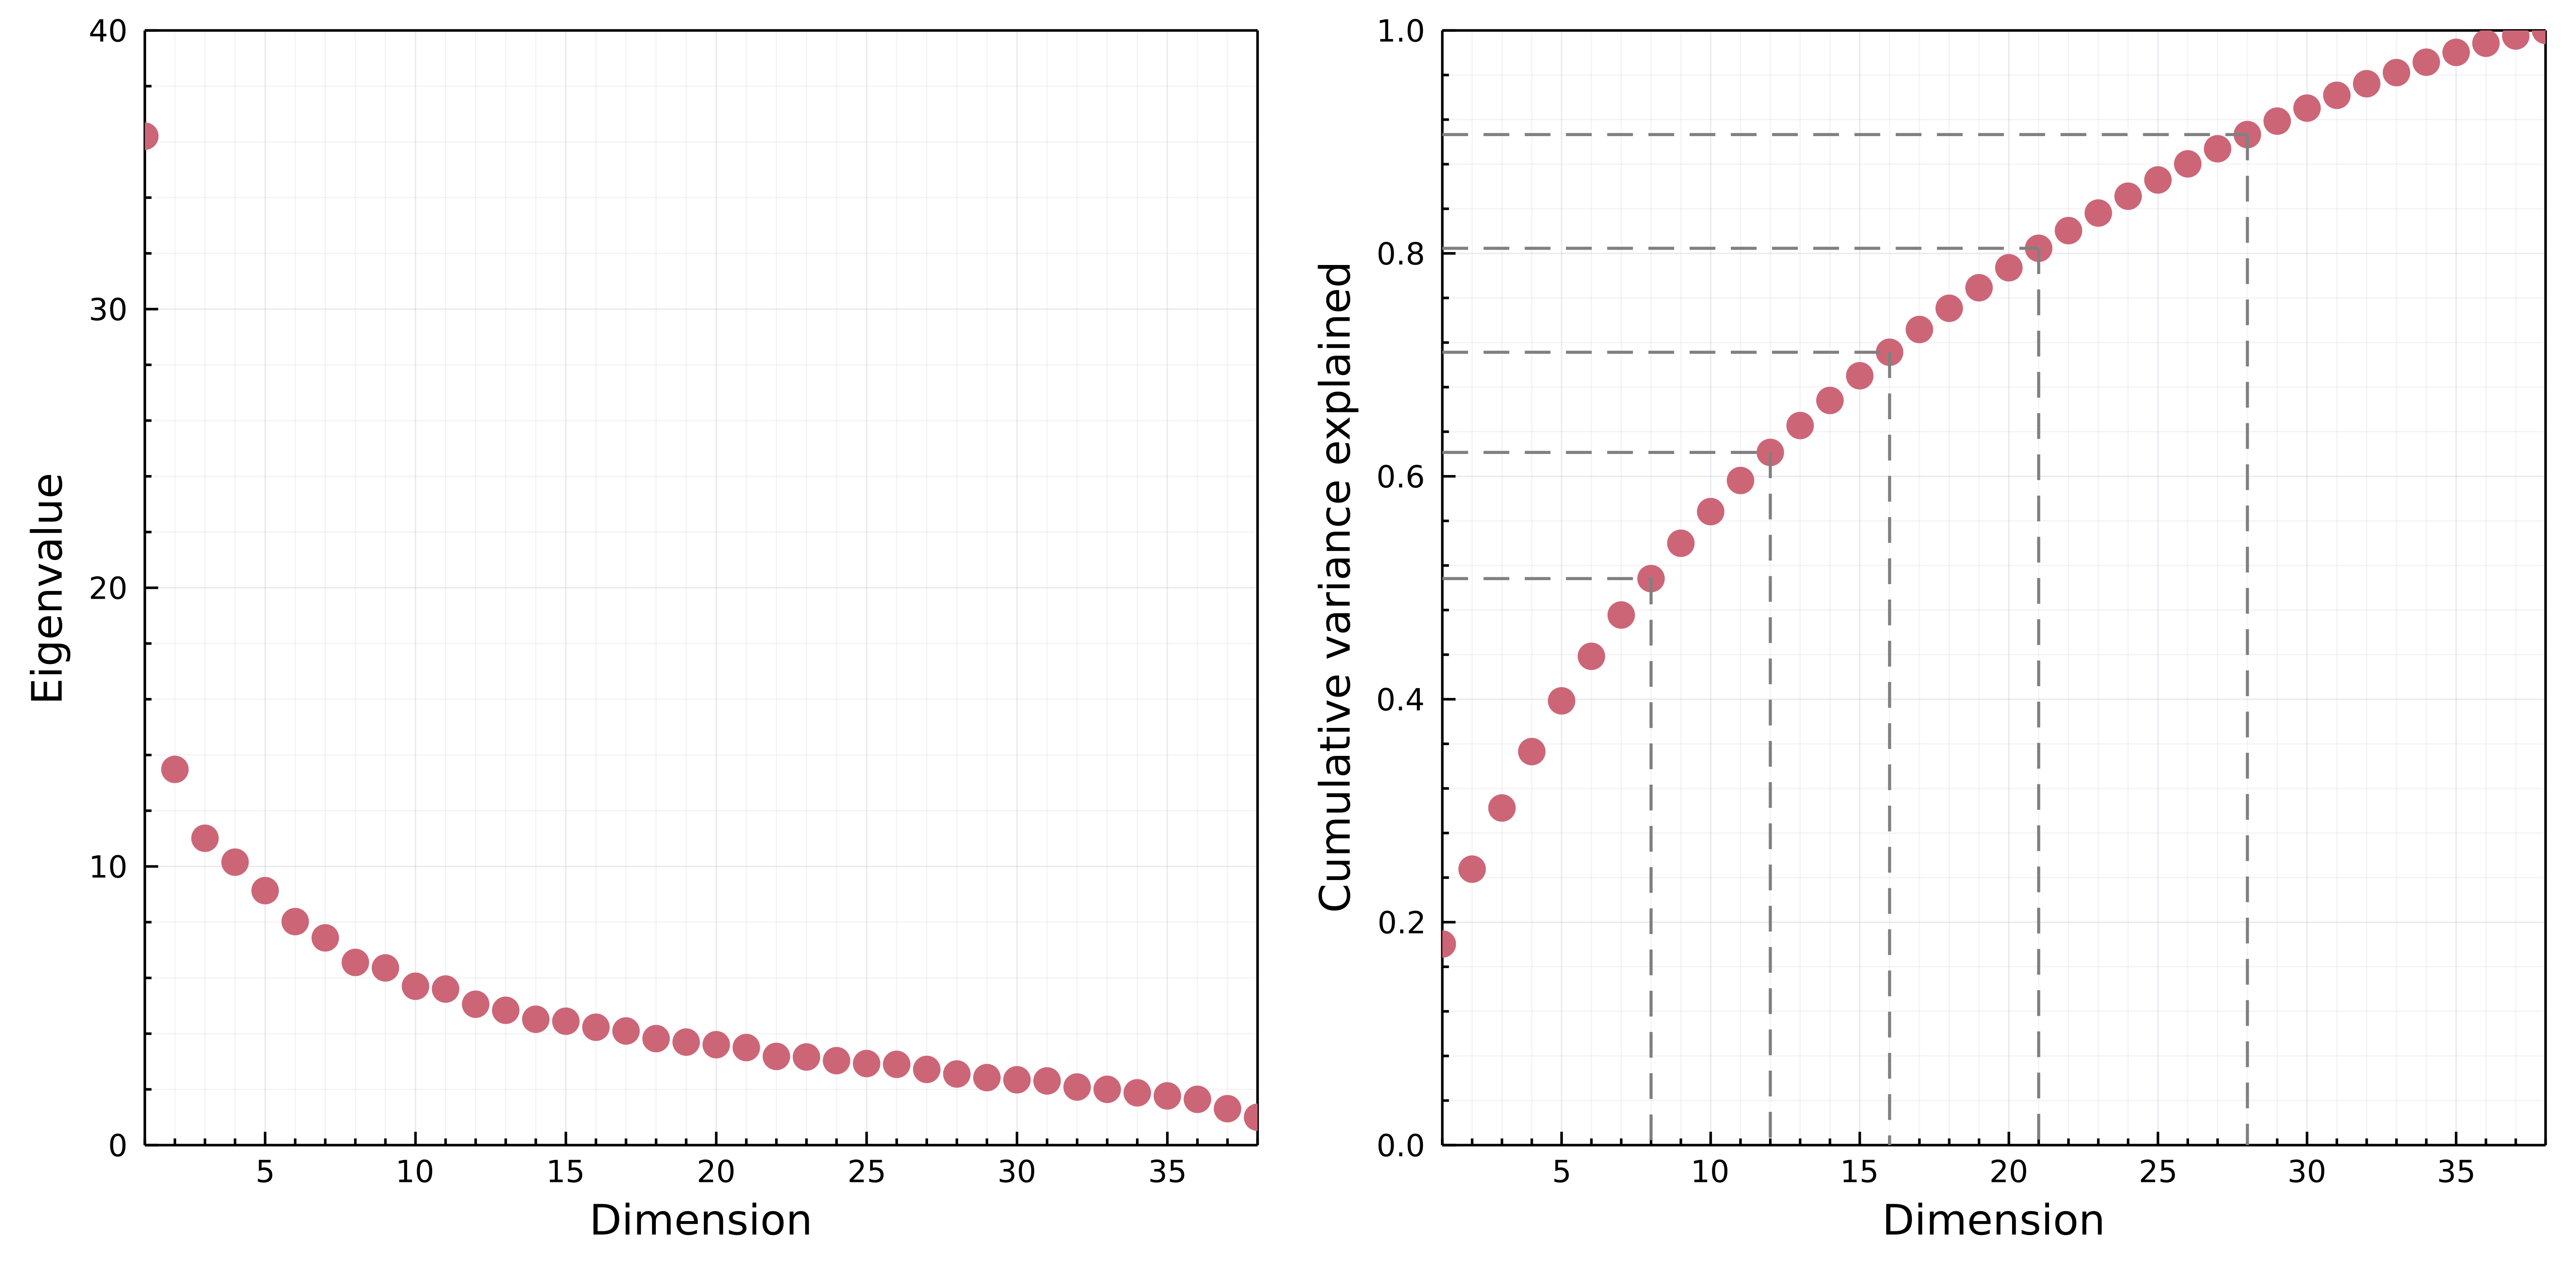
\includegraphics{figures/figure-screeplot.png}
\caption{Left: representation of the scree plot of the singular values
from the t-SVD on the European metaweb. The scree plot shows no obvious
drop in the singular values that may be leveraged to automatically
detect a minimal dimension for embedding, after \emph{e.g.} Zhu \&
Ghodsi (2006). Right: cumulative fraction of variance explained by each
dimension up to the rank of the European metaweb. The grey lines
represent cutoffs at 50, 60, \ldots, 90\% of variance explained. For the
rest of the analysis, we reverted to an arbitrary threshold of 60\% of
variance explained, which represented a good tradeoff between accuracy
and reduced number of features.}\label{fig:scree}
}
\end{figure}

Because RDPG relies on matrix multiplication, the higher dimensions
essentially serve to make specific interactions converge towards 0 or 1;
therefore, for reasonably low ranks, there is no guarantee that the
values in the reconstructed network will be within the unit range. In
order to determine what constitutes an appropriate threshold for
probability, we performed the RDPG approach on the European metaweb, and
evaluated the probability threshold by treating this as a binary
classification problem, specifically assuming that both 0 and 1 in the
European metaweb are all true. Given the methodological details given in
Maiorano et al. (2020a) and O'Connor et al. (2020), this seems like a
reasonable assumption, although one that does not hold for all metawebs.
We used the thresholding approach presented in Poisot, Ouellet, et al.
(2021), and picked a cutoff that maximized Youden's \(J\) statistic (a
measure of the informedness (trust) of predictions; Youden (1950)); the
resulting cutoff was 0.22, and gave an accuracy above 0.99. In Supp.
Mat. 1, we provide several lines of evidence that using the entire
network to estimate the threshold does not lead to overfitting; that
using a subset of species would yield the same threshold; that
decreasing the quality of the original data by adding or removing
interactions would minimally affect the predictive accuracy of RDPG
applied to the European metaweb; and that the networks reconstructed
from artificially modified data are reconstructed with the correct
ecological properties.

The left and right subspaces for the European metaweb, accompanied by
the threshold for prediction, represent the knowledge we seek to
transfer. In the next section, we explain how we rely on phylogenetic
similarity to do so.

\hypertarget{steps-2-and-3-transfer-learning-through-phylogenetic-relatedness}{%
\subsection{Steps 2 and 3: Transfer learning through phylogenetic
relatedness}\label{steps-2-and-3-transfer-learning-through-phylogenetic-relatedness}}

In order to transfer the knowledge from the European metaweb to the
Canadian species pool, we performed ancestral character estimation using
a Brownian motion model, which is a conservative approach in the absence
of strong hypotheses about the nature of phylogenetic signal in the
network decomposition (Litsios \& Salamin, 2012). This uses the
estimated feature vectors for the European mammals to create a state
reconstruction for all species (conceptually something akin to a
trait-based mammalian phylogeny using latent generality and
vulnerability traits) and allows us to impute the missing (latent) trait
data for the Canadian species that are not already in the European
network; as we are focused on predicting contemporary interactions, we
only retained the values for the tips of the tree. We assumed that all
traits (\emph{i.e.} the feature vectors for the left and right
subspaces) were independent, which is a reasonable assumption as every
trait/dimension added to the t-SVD has an \emph{additive} effect to the
one before it. Note that the Upham et al. (2019) tree itself has some
uncertainty associated to inner nodes of the phylogeny. In this case
study we have decided to not propagate this uncertainty as it would
complexify the process. The Brownian motion algorithm returns the
\emph{average} value of the trait, and its upper and lower bounds.
Because we do not estimate other parameters of the traits'
distributions, we considered that every species trait is represented as
a uniform distribution between these bounds. The choice of the uniform
distribution was made because the algorithm returns a minimum and
maximum point estimate for the value, and given this information, the
uniform distribution is the one with maximum entropy. Had all mean
parameters estimates been positive, the exponential distribution would
have been an alternative, but this is not the case for the subspaces of
an RDPG. In order to examine the consequences of the choice of
distribution, we estimated the variance per latent variable per node to
use a Normal distribution; as we show in Supp. Mat. 2, this decision
results in dramatically over-estimating the number and probability of
interactions, and therefore we keep the discussions in the main text to
the uniform case. The inferred left and right subspaces for the Canadian
species pool (\(\hat{\mathscr{L}}\) and \(\hat{\mathscr{R}}\)) have
entries that are distributions, representing the range of values for a
given species at a given dimension. These objects represent the
transferred knowledge, which we can use for prediction of the Canadian
metaweb.

\hypertarget{step-4-probabilistic-prediction-of-the-destination-network}{%
\subsection{Step 4: Probabilistic prediction of the destination
network}\label{step-4-probabilistic-prediction-of-the-destination-network}}

The phylogenetic reconstruction of \(\hat{\mathscr{L}}\) and
\(\hat{\mathscr{R}}\) has an associated uncertainty, represented by the
breadth of the uniform distribution associated to each of their entries.
Therefore, we can use this information to assemble a
\emph{probabilistic} metaweb in the sense of Poisot et al. (2016),
\emph{i.e.} in which every interaction is represented as a single,
independent, Bernoulli event of probability \(p\).

\begin{figure}
\hypertarget{fig:subspaces}{%
\centering
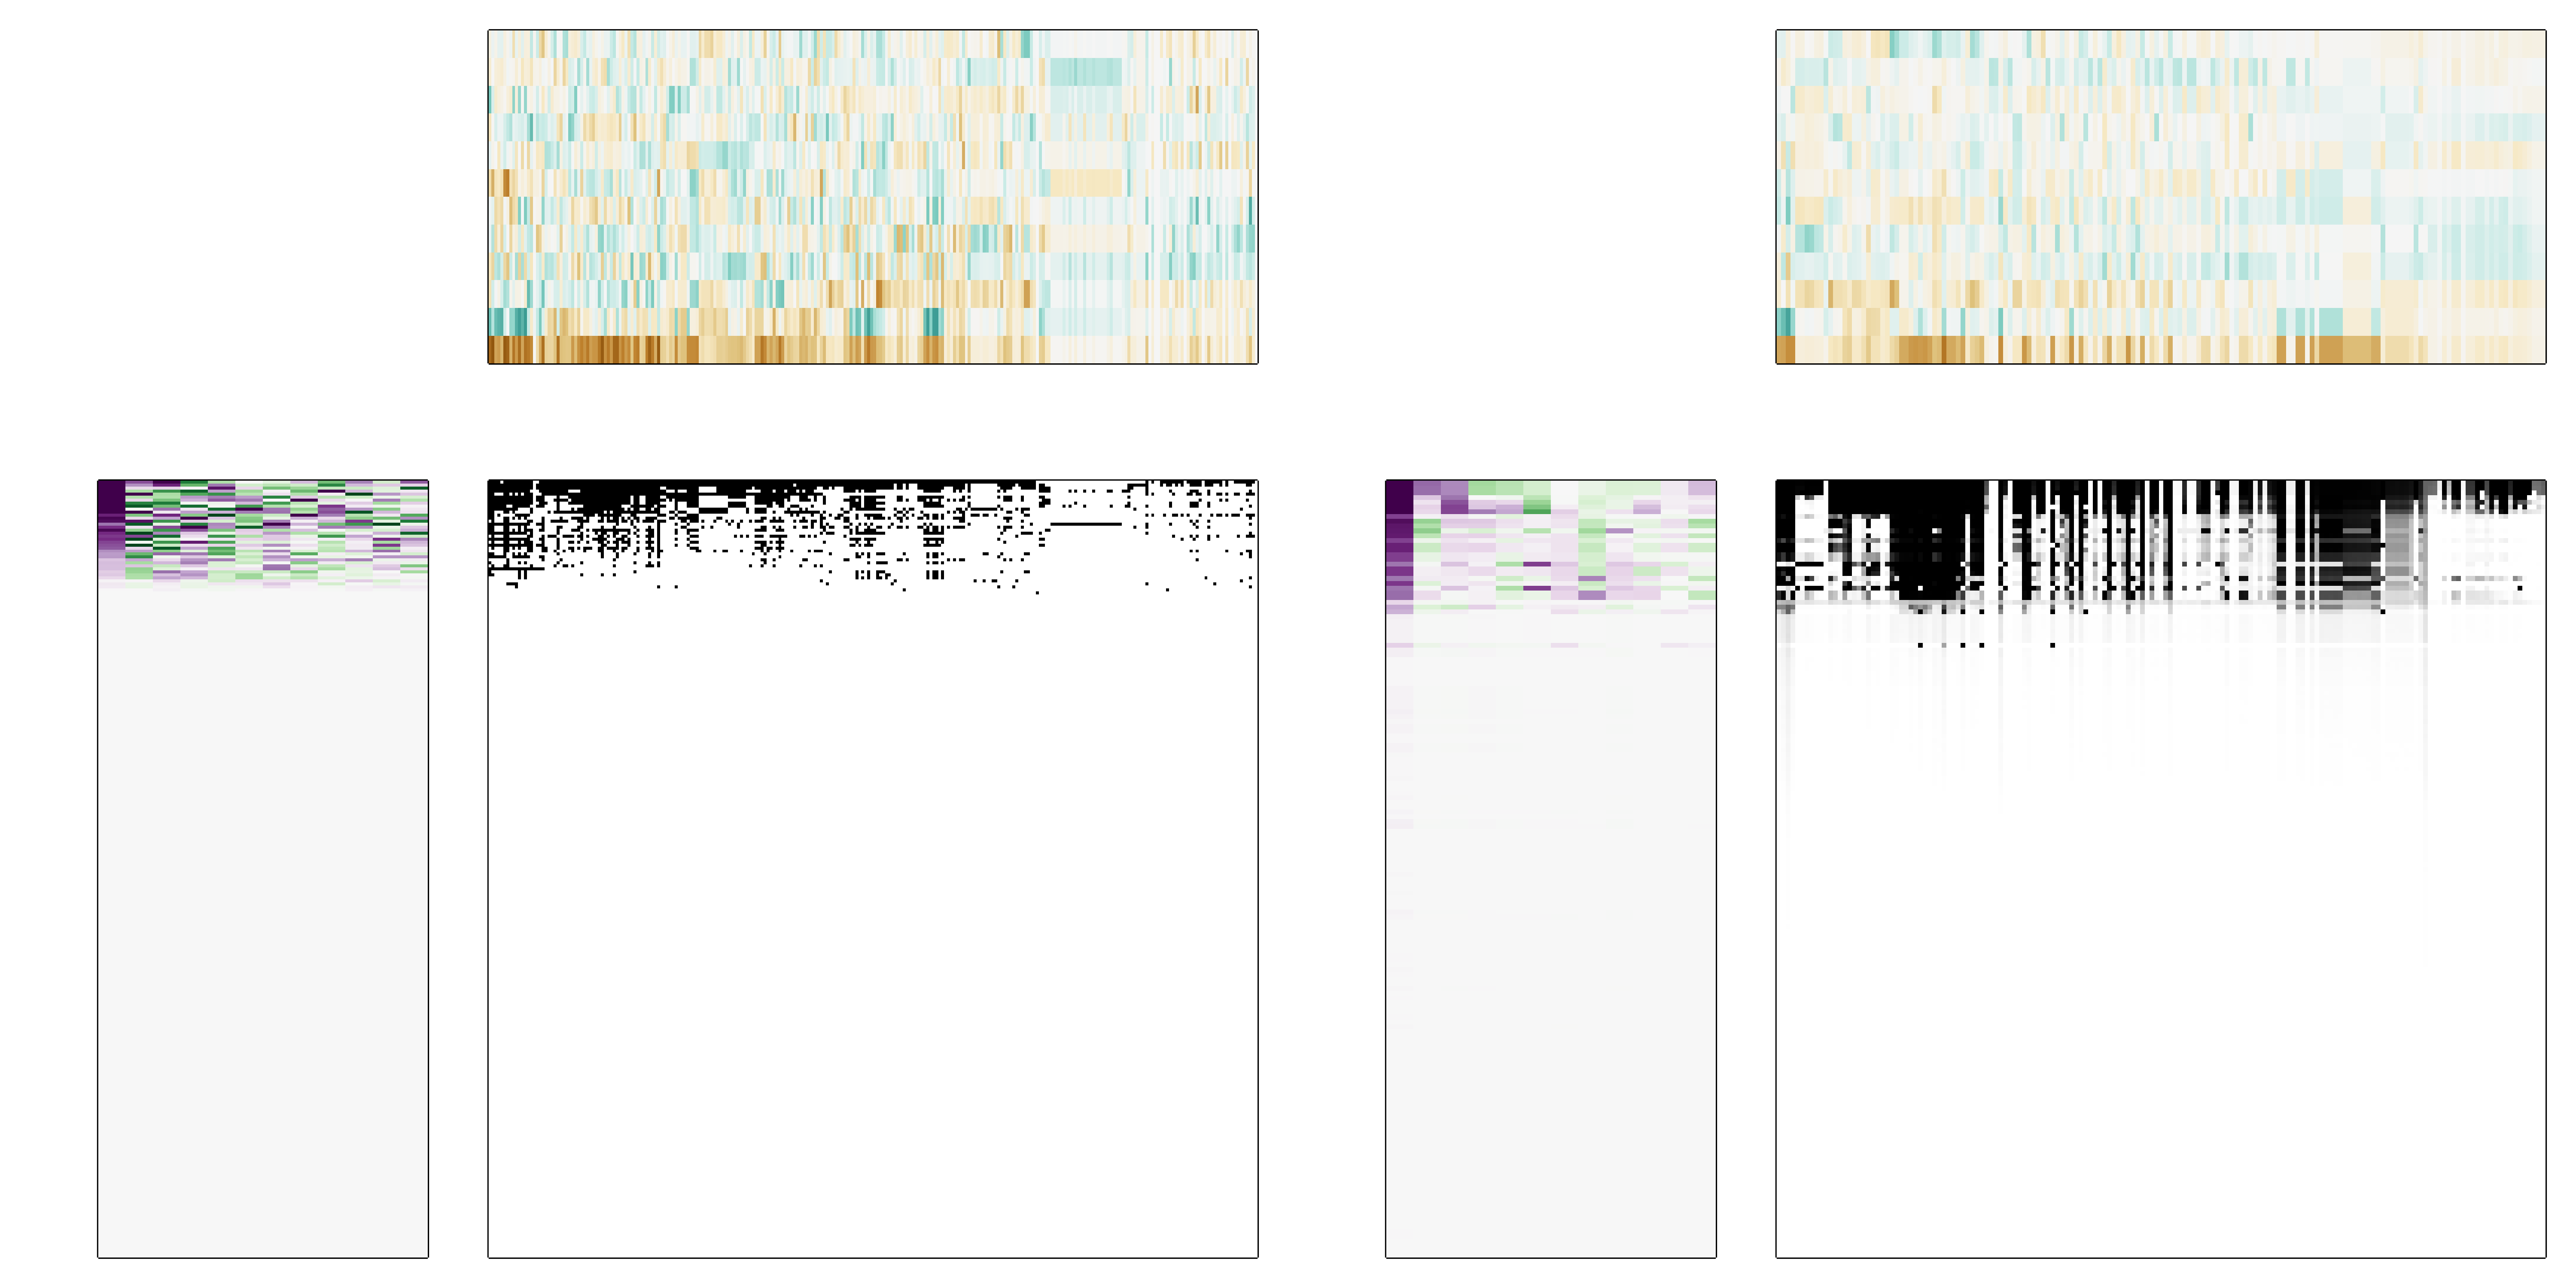
\includegraphics{figures/figure-subspaces.png}
\caption{Visual representation of the left (green/purple; left-side
matrix) and right (green/brown; top matrix) subspaces, alongside the
adjacency matrix of the food web they encode (greyscale). The European
metaweb is on the left, and the imputed Canadian metaweb (before data
inflation) on the right. This figure illustrates how much structure the
left subspace captures. As we show in fig.~\ref{fig:degree}, the species
with a value of 0 in the left subspace are species without any
prey.}\label{fig:subspaces}
}
\end{figure}

Specifically, we have adopted the following approach. For every entry in
\(\hat{\mathscr{L}}\) and \(\hat{\mathscr{R}}\), we draw a value from
its distribution. This results in one instance of the possible left
(\(\hat{\mathscr{l}}\)) and right (\(\hat{\mathscr{r}}\)) subspaces for
the Canadian metaweb. These can be multiplied, to produce one matrix of
real values. Because the entries in \(\hat{\mathscr{l}}\) and
\(\hat{\mathscr{r}}\) are in the same space where \(\mathscr{L}\) and
\(\mathscr{R}\) were originally predicted, it follows that the threshold
\(\rho\) estimated for the European metaweb also applies. We use this
information to produce one random Canadian metaweb,
\(N = \hat{\mathscr{L}}\hat{\mathscr{R}}' \ge \rho\). As we can see in
(fig.~\ref{fig:subspaces}), the European and Canadian metawebs are
structurally similar (as would be expected given the biogeographic
similarities) and the two (left and right) subspaces are distinct
\emph{i.e.} capturing predation (generality) and prey (vulnerability)
latent traits.

Because the intervals around some trait values can be broad (in fact,
probably broader than what they would actually be, see \emph{e.g.}
Garland et al., 1999), we repeat the above process \(2\times 10^5\)
times, which results in a probabilistic metaweb \(P\), where the
probability of an interaction (here conveying our degree of trust that
it exists given the inferred trait distributions) is given by the number
of times where it appears across all random draws \(N\), divided by the
number of samples. An interaction with \(P_{i,j} = 1\) means that these
two species were predicted to interact in all \(2\times 10^5\) random
draws.

It must be noted that despite bringing in a large amount of information
from the European species pool and interactions, the Canadian metaweb
has distinct structural properties. Following an approach similar to
Vermaat et al. (2009), we show in Supp. Mat. 3 that not only can we
observe differences in the multivariate space between the European and
Canadian metawebs, we can also observe differences in the same space
between random subgraphs from these networks. These results line up with
the studies spatializing metawebs that have been discussed in the
introduction: changes in the species pool are driving local structural
changes in the networks.

\hypertarget{data-cleanup-discovery-validation-and-thresholding}{%
\subsection{Data cleanup, discovery, validation, and
thresholding}\label{data-cleanup-discovery-validation-and-thresholding}}

Once the probabilistic metaweb for Canada has been produced, we followed
a number of data inflation steps to finalize it. This step is external
to the actual transfer learning framework but rather serves as a way to
augment and validate the predicted metaweb.

\begin{figure}
\hypertarget{fig:inflation}{%
\centering
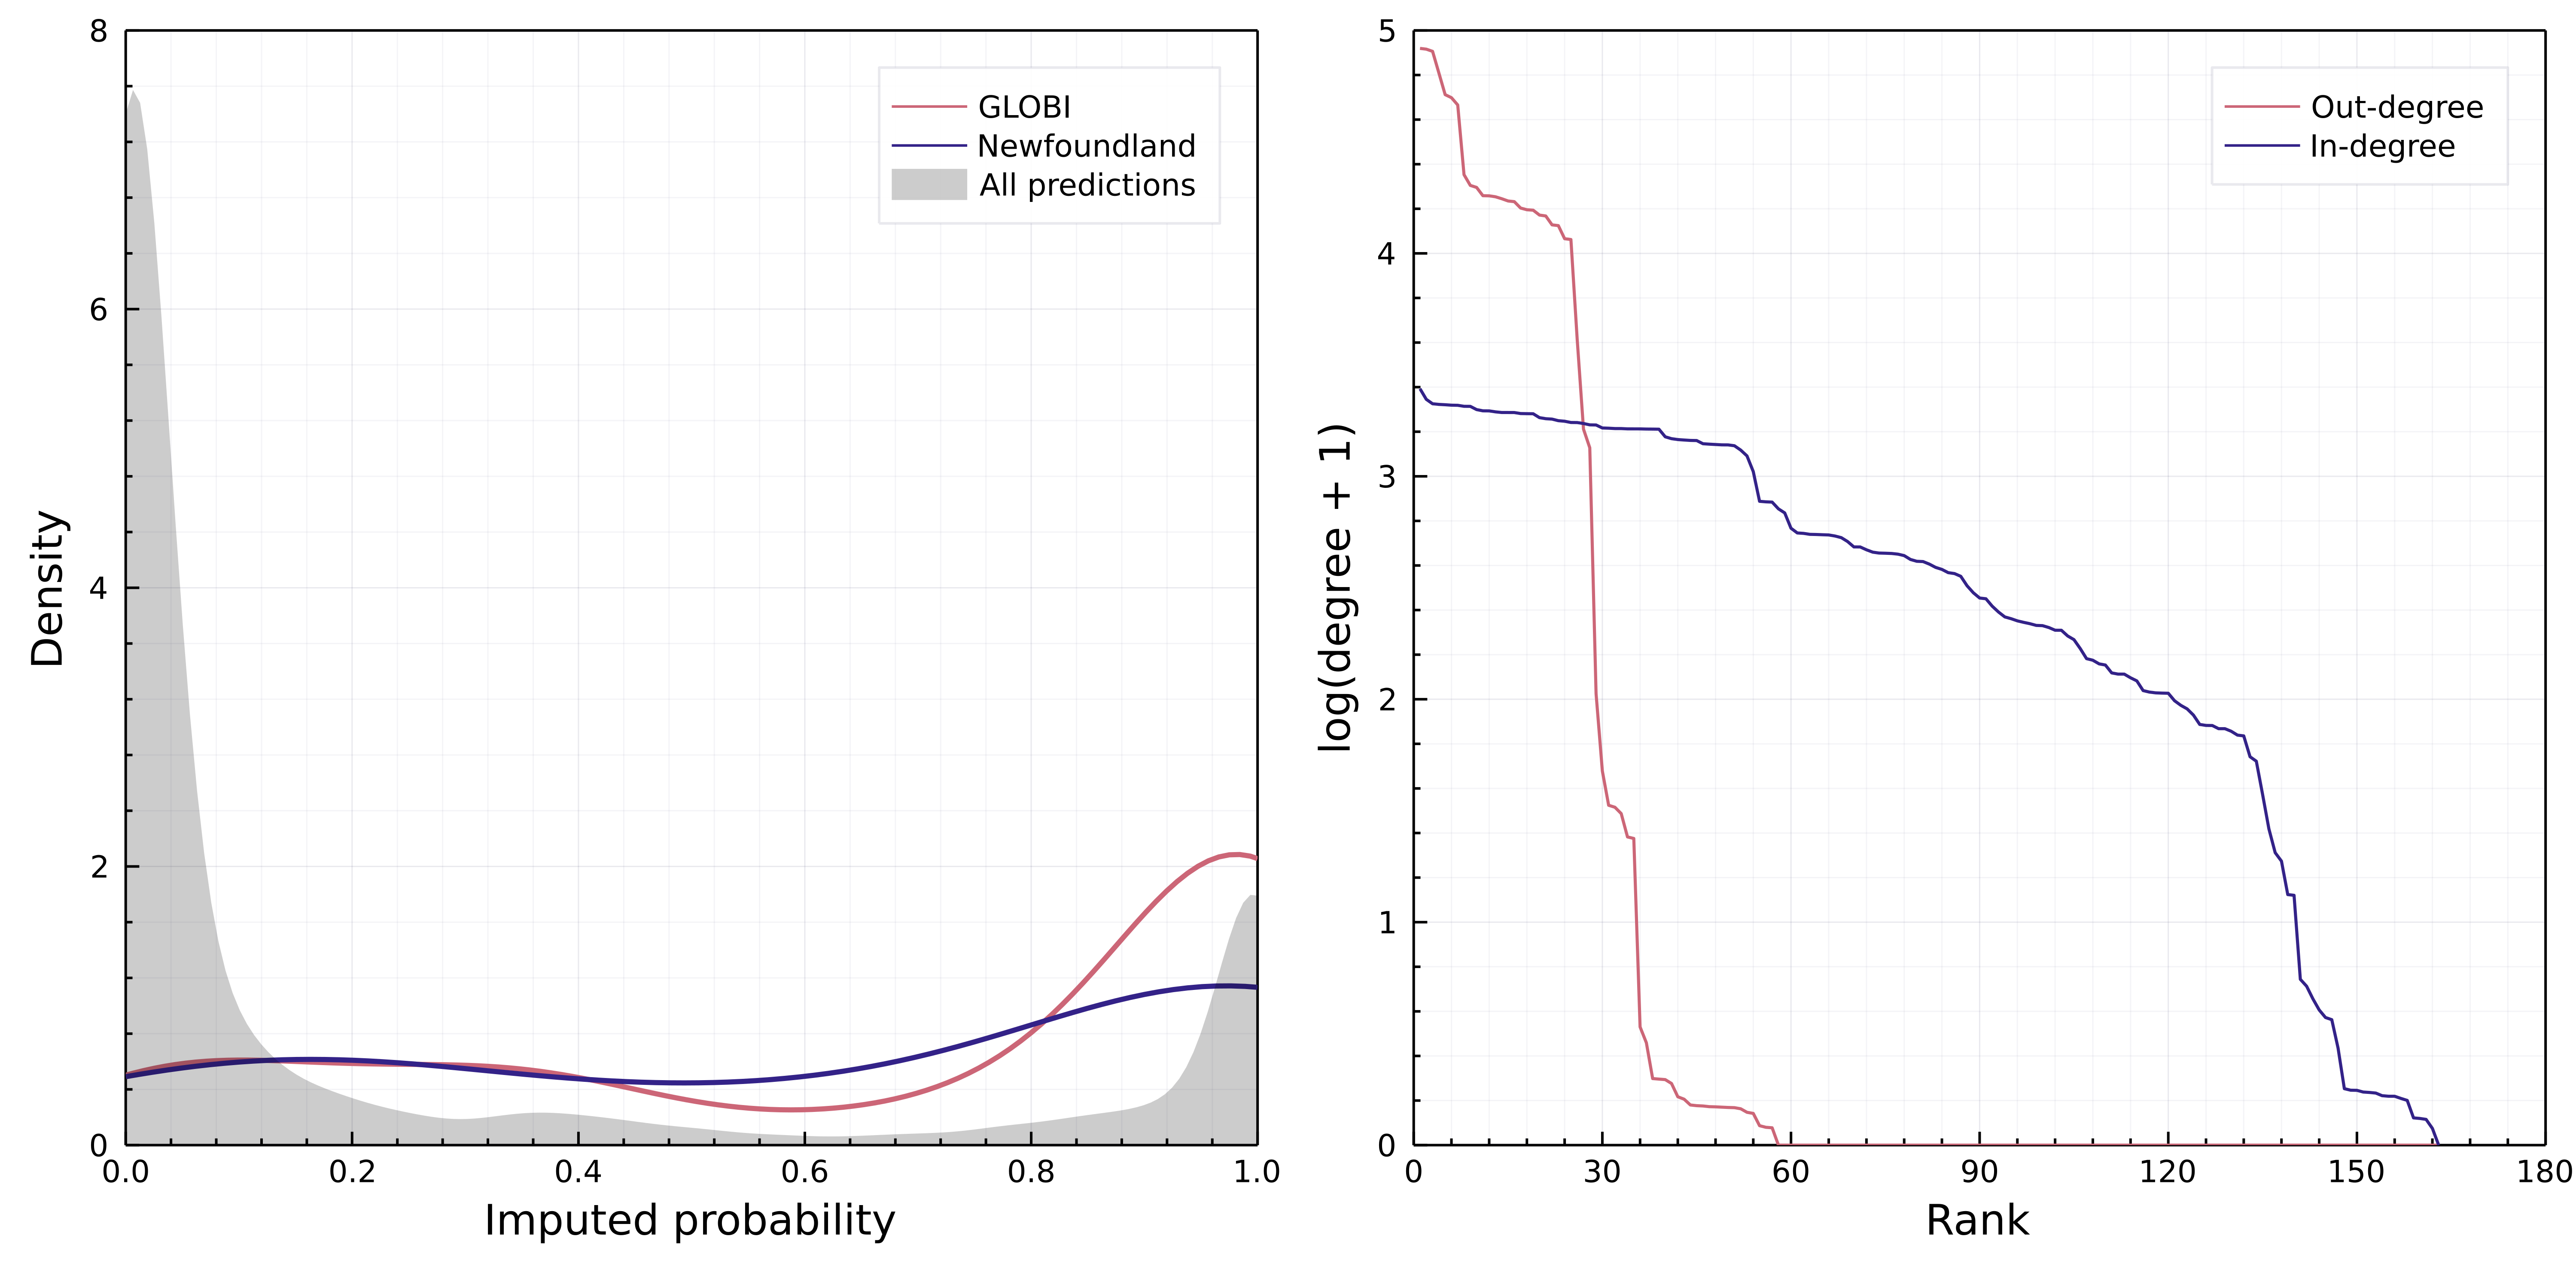
\includegraphics{figures/figure-validation.png}
\caption{Left: comparison of the probabilities of interactions assigned
by the model to all interactions (grey curve), the subset of
interactions found in GloBI (red), and in the Strong \& Leroux (2014)
Newfoundland dataset (blue). The model recovers more interactions with a
low probability compared to data mining, which can suggest that
collected datasets are biased towards more common or easy to identify
interactions. Right: distribution of the in-degree and out-degree of the
mammals from Canada in the reconstructed metaweb. This figure describes
a flat, relatively short food web, in which there are few predators but
a large number of preys.}\label{fig:inflation}
}
\end{figure}

First, we extracted the network corresponding to the 17 species shared
between the European and Canadian pools and replaced these interactions
with a probability of 0 (non-interaction) or 1 (interaction), according
to their value in the European metaweb. This represents a minute
modification of the inferred network (about 0.8\% of all species pairs
from the Canadian web), but ensures that we are directly re-using
knowledge from Europe.

Second, we looked for all species in the Canadian pool known to the
Global Biotic Interactions (GloBI) database (Poelen et al., 2014), and
extracted their known interactions. Because GloBI aggregates observed
interactions, it is not a \emph{networks} data source, and therefore the
only information we can reliably extract from it is that a species pair
\emph{was reported to interact at least once}. This last statement
should yet be taken with caution, as some sources in GloBI (\emph{e.g.}
Thessen \& Parr, 2014) are produced through text analysis, and therefore
may not document direct evidence of the interaction. Nevertheless,
should the predictive model work, we would expect that a majority of
interactions known to GloBI would also be predicted. We retrieved 366
interactions between mammals from the Canadian species pool from GloBI,
33 of which were not predicted by the model; this results in a success
rate of 91\%. After performing this check, we set the probability of all
interactions known to GloBI to 1.

Finally, we downloaded the data from Strong \& Leroux (2014), who mined
various literature sources to identify trophic interactions in
Newfoundland. This dataset documented 25 interactions between mammals,
only two of which were not part of our (Canada-level) predictions,
resulting in a success rate of 92\%. These two interactions were added
to our predicted metaweb with a probability of 1. A comparison of
interaction densities for the inferred metaweb, and the Globi and
Newfoundland is shown in fig.~\ref{fig:inflation} and a table listing
all interactions in the predicted Canadian metaweb can be found in the
supplementary material.

\begin{figure}
\hypertarget{fig:thresholds}{%
\centering
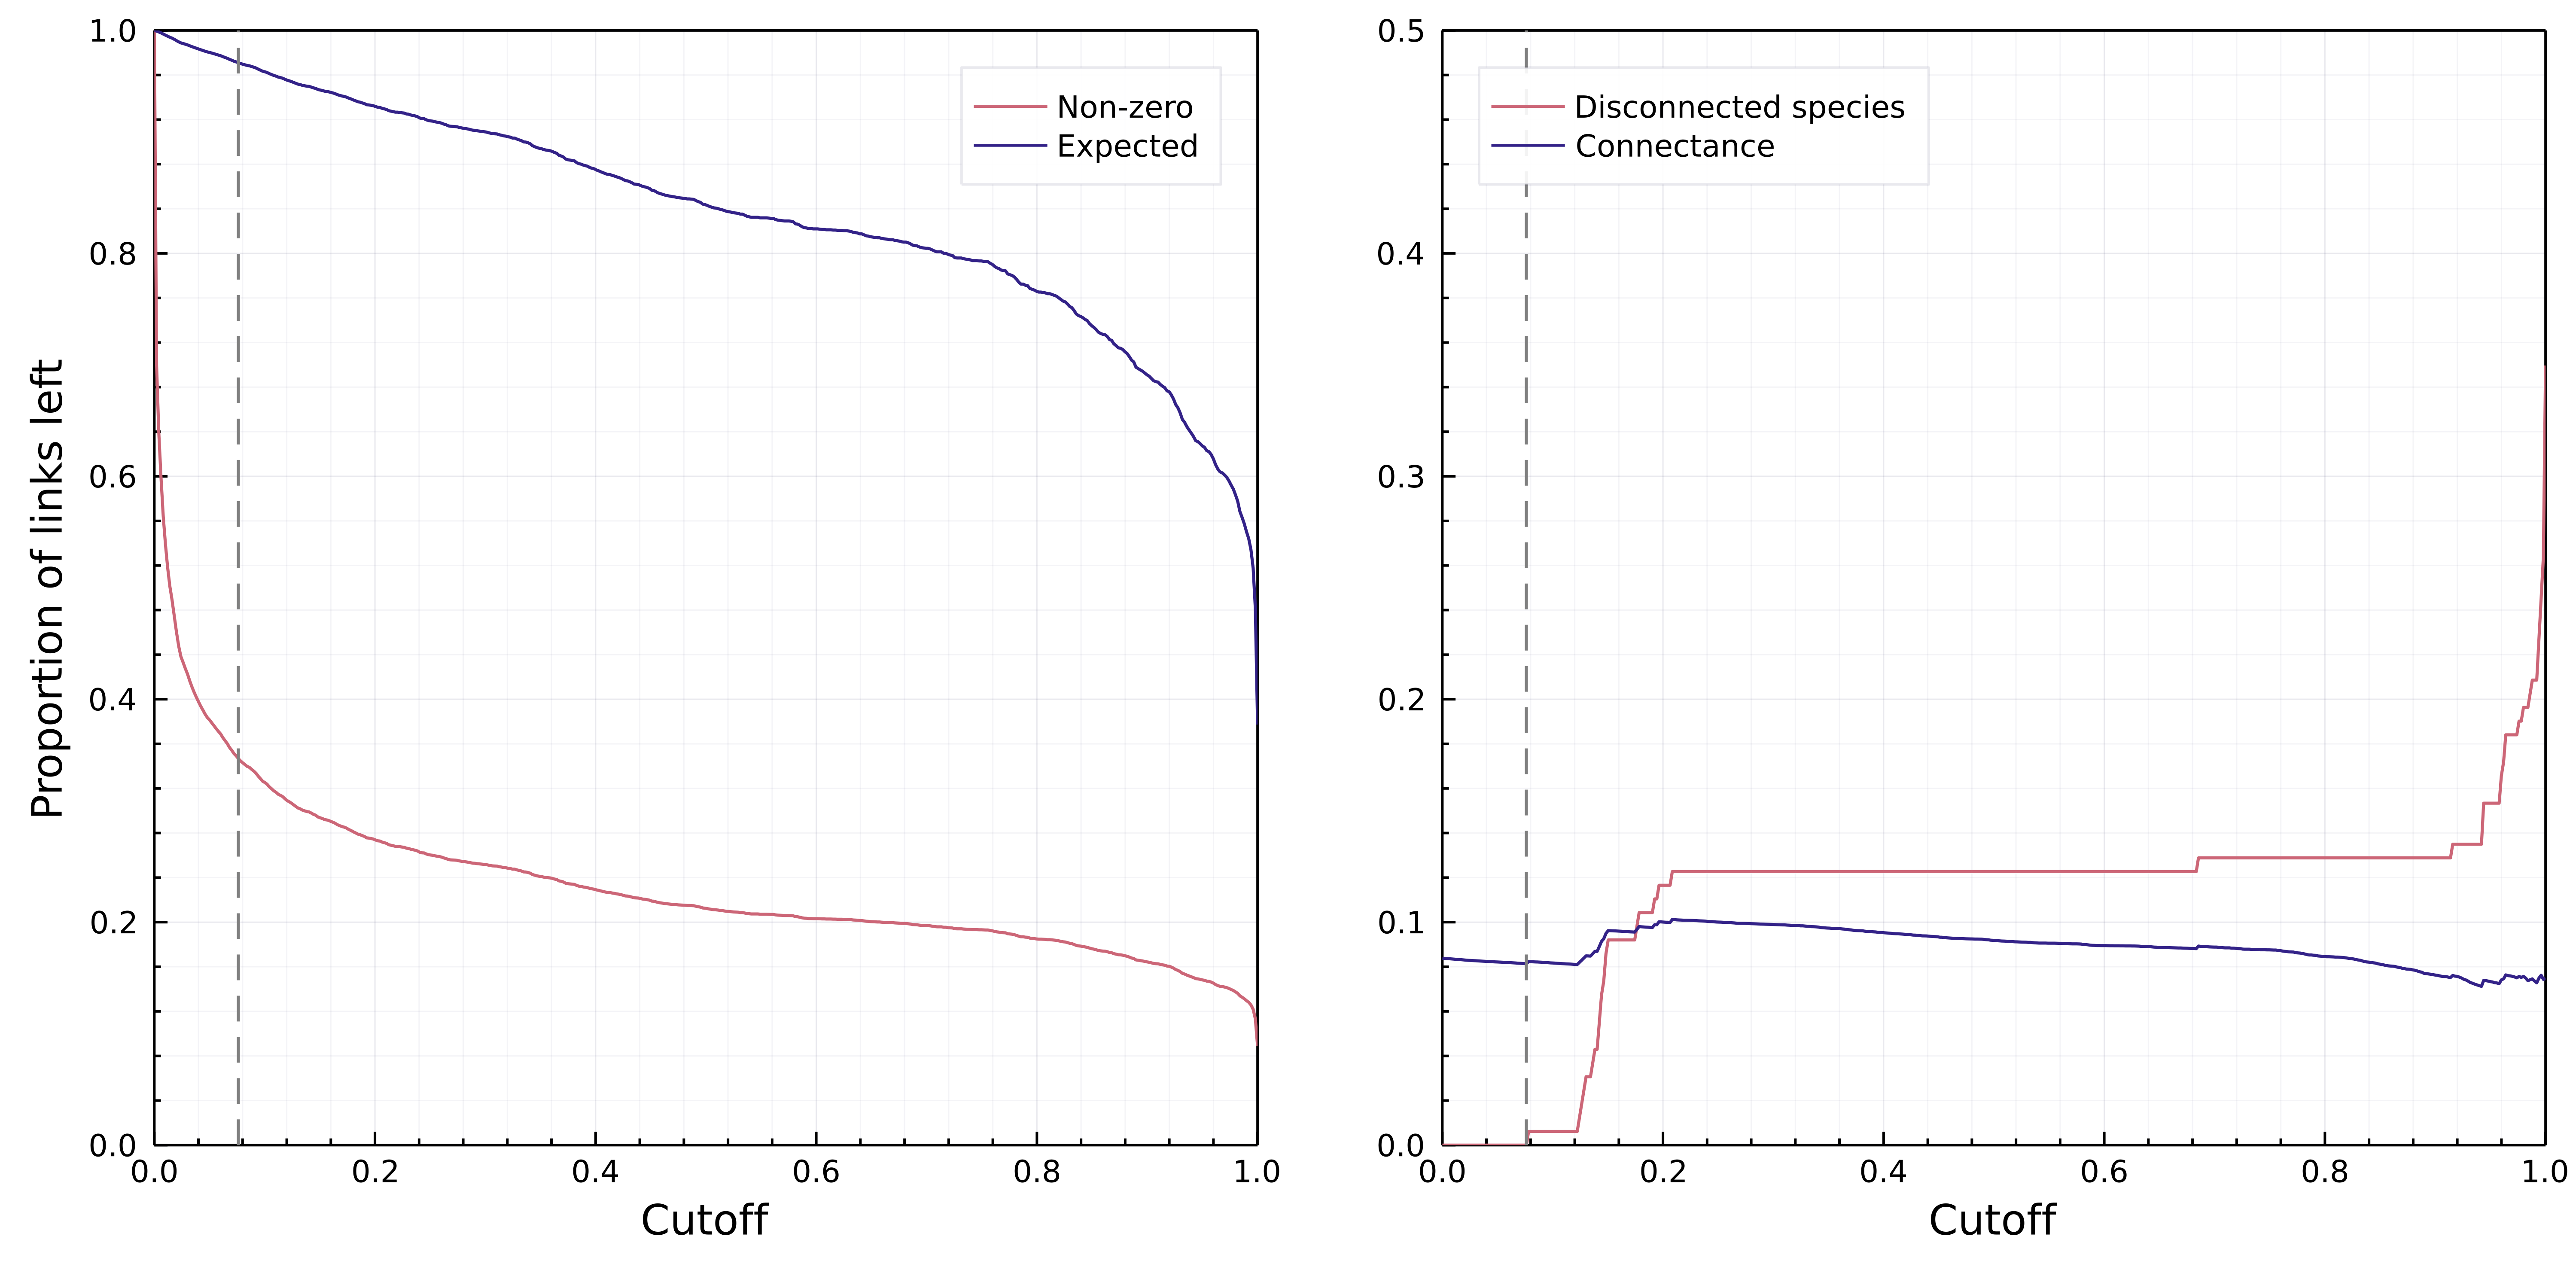
\includegraphics{figures/figure-cutoffs.png}
\caption{Left: effect of varying the cutoff for probabilities to be
considered non-zero on the number of unique links and on \(\hat{L}\),
the probabilistic estimate of the number of links assuming that all
interactions are independent. Right: effect of varying the cutoff on the
number of disconnected species, and on network connectance. In both
panels, the grey line indicates the cutoff
\(P(i\rightarrow j) \approx 0.08\) that resulted in the first species
losing all of its interactions.}\label{fig:thresholds}
}
\end{figure}

Because the confidence intervals on the inferred trait space are
probably over-estimates, we decided to apply a thresholding step to the
interactions after data inflation (see fig.~\ref{fig:thresholds} showing
the effect of varying the cutoff on \(P(i \rightarrow j)\)). Cirtwill \&
Hambäck (2021) proposed a number of strategies to threshold
probabilistic networks. Their methodology assumes the underlying data to
be tag-based sequencing, which represents interactions as co-occurrences
of predator and prey within the same tags; this is conceptually
identical to our Bernoulli-trial based reconstruction of a probabilistic
network. We performed a full analysis of the effect of various cutoffs,
and as they either resulted in removing too few interactions, or
removing enough interactions that species started to be disconnected
from the network, we set this threshold for a probability equivalent to
0 to the largest possible value that still allowed all species to have
at least one interaction with a non-zero probability. The need for this
slight deviation from the Cirtwill \& Hambäck (2021) methodology
highlights the need for additional development on network thresholding.

\hypertarget{results-and-discussion}{%
\section{Results and discussion}\label{results-and-discussion}}

\begin{figure}
\hypertarget{fig:degree}{%
\centering
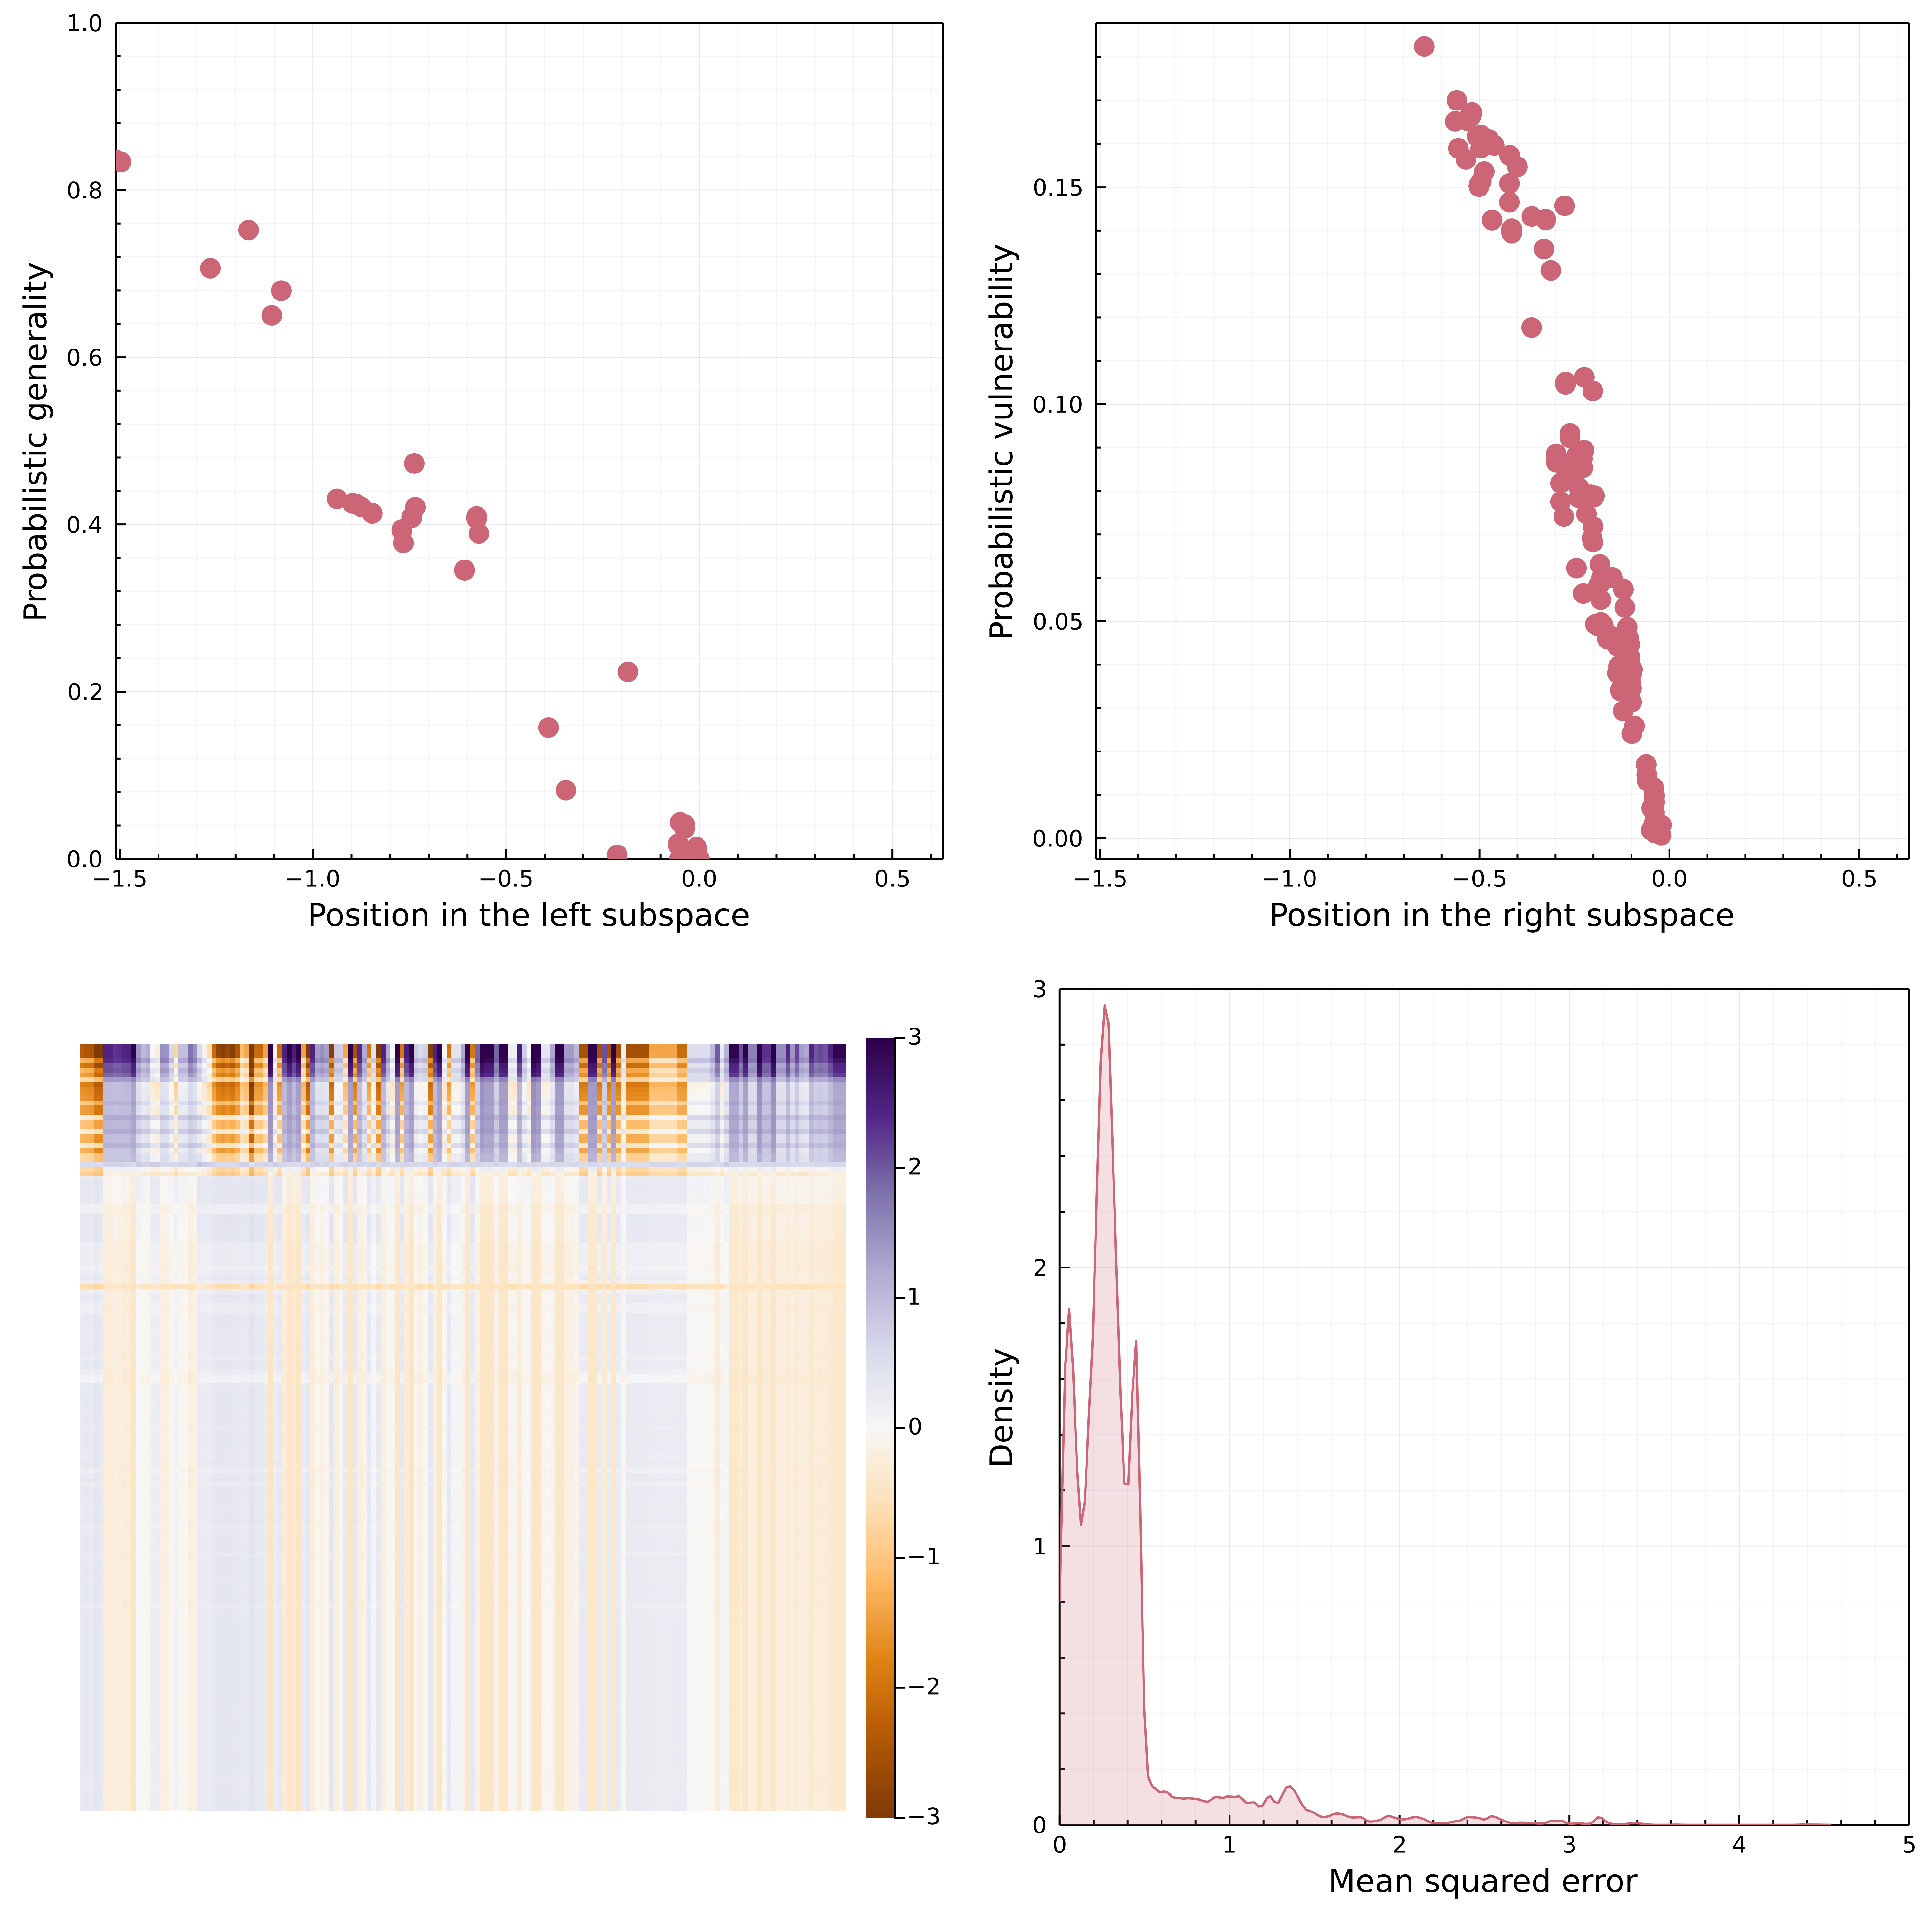
\includegraphics{figures/figure-degree.png}
\caption{Top: biological significance of the first dimension. Left:
there is a linear relationship between the values on the first dimension
of the left subspace and the generality, \emph{i.e.} the relative number
of preys, \emph{sensu} Schoener (1989). Species with a value of 0 in
this subspace are at the bottom-most trophic level. Right: there is,
similarly, a linear relationship between the position of a species on
the first dimension of the right subspace and its vulnerability,
\emph{i.e.} the relative number of predators. Taken together, these two
figures show that the first-order representation of this network would
capture its degree distribution. Bottom: topological consequences of the
first dimension. Left: differences in the \(z\)-scores of the actual
configuration model for the reconstructed network, and the prediction
based only on the first dimension. Right: distribution of the
differences in the left panel.}\label{fig:degree}
}
\end{figure}

Using a transfer learning framework we were able to construct a
probabilistic metaweb and (as per Dunne, 2006) is a list of potential
interactions, meaning that they will not necessarily be realized
wherever the two species co-occur. The t-SVD embedding is able to learn
relevant ecological features for the network. fig.~\ref{fig:degree}
shows that the first rank correlates linearly with generality and
vulnerability (Schoener, 1989), \emph{i.e.} the number of preys and
predators for each species. Importantly, this implies that a rank 1
approximation represents the configuration model for the metaweb,
\emph{i.e.} a set of random networks generated from a given degree
sequence (Park \& Newman, 2004). Accounting for the probabilistic nature
of the degrees, the rank 1 approximation also represents the \emph{soft}
configuration model (van der Hoorn et al., 2018). Both models are
maximum entropy graph models (Garlaschelli et al., 2018), with sharp
(all network realizations satisfy the specified degree sequence) and
soft (network realizations satisfy the degree sequence on average) local
constraints, respectively. The (soft) configuration model is an unbiased
random graph model widely used by ecologists in the context of null
hypothesis significance testing of network structure (\emph{e.g.}
Bascompte et al., 2003) and can provide informative priors for Bayesian
inference of network structure (\emph{e.g.} J.-G. Young et al., 2021).
It is noteworthy that for this metaweb, the relevant information was
extracted at the first rank. Because the first rank corresponds to the
leading singular value of the system, the results of
fig.~\ref{fig:degree} have a straightforward interpretation:
degree-based processes are the most important in structuring the
mammalian food web.

One important aspect in which Europe and Canada differ (despite their
comparable bioclimatic conditions) is the degree of the legacy of human
impacts, which have been much longer in Europe. Nenzén et al. (2014)
showed that even at small scales (the Iberian peninsula), mammal food
webs retain the signal of both past climate change and human activity,
even when this human activity was orders of magnitude less important
than it is now. Similarly, Yeakel et al. (2014) showed that changes in
human occupation over several centuries can lead to food web collapse.
Megafauna in particular seems to be very sensitive to human arrival
(Pires et al., 2015). In short, there is well-substantiated support for
the idea that human footprint affects more than the risk of species
extinction (Marco et al., 2018), and can lead to changes in interaction
structure.

Cirtwill et al. (2019) showed that network inference techniques based on
Bayesian approaches would perform far better in the presence of an
interaction-level informative prior; the desirable properties of such a
prior would be that it is expressed as a probability, preferably
representing a Bernoulli event, the value of which would be
representative of relevant biological processes (probability of
predation in this case). We argue that the probability returned at the
very last step of our framework may serve as this informative prior;
indeed, the output of our analysis can be used in subsequent steps, also
possibly involving expert elicitation to validate some of the most
strongly recommended interactions. One important \emph{caveat} to keep
in mind when working with interaction inference is that interactions can
never really be true negatives (in the current state of our
methodological framework and data collection limitations); this renders
the task of validating a model through the usual application of binary
classification statistics very difficult (although see Strydom, Catchen,
et al., 2021 for a discussion of alternative suggestions). The other way
through which our framework can be improved is by substituting the
predictors that are used for transfer. For example, in the presence of
information on species traits that are known to be predictive of species
interactions, one might want to rely on functional rather than
phylogenetic distances -- in food webs, body size (and allometrically
related variables) has been established as such a variable (Brose et
al., 2006); the identification of relevant functional traits is
facilitated by recent methodological developments (Rosado et al., 2013).

Finally, it should be noted that the framework we have presented is
amenable to changes lending to applicability to a broad range of
potential scenarios. For example in this case study we have embedded the
original metaweb using t-SVD, because it lends itself to an RDPG
reconstruction, which is known to capture the consequences of
evolutionary processes (Dalla Riva \& Stouffer, 2016); this being said,
there are other ways to embed graphs (Arsov \& Mirceva, 2019; Cai et
al., 2017; Cao et al., 2019), which can be used as alternatives.
Regarding the transfer step it is possible to use distinct trees if
working with distinct clades (such as pollination networks) or an
alternative measure of similarity (transfer medium) such as information
on foraging (Beckerman et al., 2006), cell-level mechanisms (Boeckaerts
et al., 2021), or a combination of traits and phylogenetic structure
(Stock, 2021). Most importantly, although we focus on a trophic system,
it is an established fact that different (non-trophic) interactions do
themselves interact with and influence the outcome of trophic
interactions (see \emph{e.g.} Kawatsu et al., 2021; Kéfi et al., 2012).
Future development of metaweb inference techniques should cover the
prediction of multiple interaction types.

\textbf{Acknowledgements:} We acknowledge that this study was conducted
on land within the traditional unceded territory of the Saint Lawrence
Iroquoian, Anishinabewaki, Mohawk, Huron-Wendat, and Omàmiwininiwak
nations. TP, TS, DC, and LP received funding from the Canadian Institute
for Ecology \& Evolution. FB is funded by the Institute for Data
Valorization (IVADO). TS, SB, and TP are funded by a donation from the
Courtois Foundation. CB was awarded a Mitacs Elevate Fellowship no.
IT12391, in partnership with fRI Research, and also acknowledges funding
from Alberta Innovates and the Forest Resources Improvement Association
of Alberta. M-JF acknowledges funding from NSERC Discovery Grant and
NSERC CRC. RR is funded by New Zealand's Biological Heritage Ngā Koiora
Tuku Iho National Science Challenge, administered by New Zealand
Ministry of Business, Innovation, and Employment. BM is funded by the
NSERC Alexander Graham Bell Canada Graduate Scholarship and the FRQNT
master's scholarship. LP acknowledges funding from NSERC Discovery Grant
(NSERC RGPIN-2019-05771). TP acknowledges financial support from NSERC
through the Discovery Grants and Discovery Accelerator Supplement
programs. MJF is supported by an NSERC PDF and an RBC Post-Doctoral
Fellowship

\textbf{Conflict of interest:} The authors have no conflict interests to
disclose

\textbf{Authors' contributions:} TS, SB, and TP designed the study and
performed the analysis; GVDR, MF, and RR provided additional feedback on
the analyses. DC, BM, and FB helped with data collection. All authors
contributed to writing and editing the manuscript.

\textbf{Data availability:} All code and data used in this manuscript is
publicly available and archived on OSF \url{https://osf.io/2zwqm/} and
is currently referenced in the manuscript.

\hypertarget{references}{%
\section*{References}\label{references}}
\addcontentsline{toc}{section}{References}

\hypertarget{refs}{}
\begin{CSLReferences}{1}{0}
\leavevmode\hypertarget{ref-Albouy2019MarFis}{}%
Albouy, C., Archambault, P., Appeltans, W., Araújo, M. B., Beauchesne,
D., Cazelles, K., Cirtwill, A. R., Fortin, M.-J., Galiana, N., Leroux,
S. J., Pellissier, L., Poisot, T., Stouffer, D. B., Wood, S. A., \&
Gravel, D. (2019). The marine fish food web is globally connected.
\emph{Nature Ecology \& Evolution}, \emph{3}(8, 8), 1153--1161.
\url{https://doi.org/10.1038/s41559-019-0950-y}

\leavevmode\hypertarget{ref-Arsov2019NetEmb}{}%
Arsov, N., \& Mirceva, G. (2019, November 26). \emph{Network Embedding:
An Overview}. \url{http://arxiv.org/abs/1911.11726}

\leavevmode\hypertarget{ref-Banville2021ManJl}{}%
Banville, F., Vissault, S., \& Poisot, T. (2021). Mangal.jl and
EcologicalNetworks.jl: Two complementary packages for analyzing
ecological networks in Julia. \emph{Journal of Open Source Software},
\emph{6}(61), 2721. \url{https://doi.org/10.21105/joss.02721}

\leavevmode\hypertarget{ref-Bascompte2003NesAss}{}%
Bascompte, J., Jordano, P., Melian, C. J., \& Olesen, J. M. (2003). The
nested assembly of plant-animal mutualistic networks. \emph{Proceedings
of the National Academy of Sciences}, \emph{100}(16), 9383--9387.
\url{https://doi.org/10.1073/pnas.1633576100}

\leavevmode\hypertarget{ref-Beckerman2006ForBio}{}%
Beckerman, A. P., Petchey, O. L., \& Warren, P. H. (2006). Foraging
biology predicts food web complexity. \emph{Proceedings of the National
Academy of Sciences}, \emph{103}(37), 13745--13749.
\url{https://doi.org/10.1073/pnas.0603039103}

\leavevmode\hypertarget{ref-Bezanson2017JulFre}{}%
Bezanson, J., Edelman, A., Karpinski, S., \& Shah, V. (2017). Julia: A
Fresh Approach to Numerical Computing. \emph{SIAM Review}, \emph{59}(1),
65--98. \url{https://doi.org/10.1137/141000671}

\leavevmode\hypertarget{ref-Boeckaerts2021PreBac}{}%
Boeckaerts, D., Stock, M., Criel, B., Gerstmans, H., De Baets, B., \&
Briers, Y. (2021). Predicting bacteriophage hosts based on sequences of
annotated receptor-binding proteins. \emph{Scientific Reports},
\emph{11}(1, 1), 1467. \url{https://doi.org/10.1038/s41598-021-81063-4}

\leavevmode\hypertarget{ref-Braga2021PhyRec}{}%
Braga, M. P., Janz, N., Nylin, S., Ronquist, F., \& Landis, M. J.
(2021). Phylogenetic reconstruction of ancestral ecological networks
through time for pierid butterflies and their host plants. \emph{Ecology
Letters}, \emph{n/a}(n/a). \url{https://doi.org/10.1111/ele.13842}

\leavevmode\hypertarget{ref-Brose2006ConRes}{}%
Brose, U., Jonsson, T., Berlow, E. L., Warren, P., Banasek-Richter, C.,
Bersier, L.-F., Blanchard, J. L., Brey, T., Carpenter, S. R.,
Blandenier, M.-F. C., Cushing, L., Dawah, H. A., Dell, T., Edwards, F.,
Harper-Smith, S., Jacob, U., Ledger, M. E., Martinez, N. D., Memmott,
J., \ldots{} Cohen, J. E. (2006). ConsumerResource Body-Size
Relationships in Natural Food Webs. \emph{Ecology}, \emph{87}(10),
2411--2417.
\url{https://doi.org/10.1890/0012-9658(2006)87\%5B2411:CBRINF\%5D2.0.CO;2}

\leavevmode\hypertarget{ref-Cai2017ComSur}{}%
Cai, H., Zheng, V. W., \& Chang, K. C.-C. (2017). \emph{A Comprehensive
Survey of Graph Embedding: Problems, Techniques and Applications}.
\url{http://arxiv.org/abs/1709.07604}

\leavevmode\hypertarget{ref-Cameron2019UneGlo}{}%
Cameron, E. K., Sundqvist, M. K., Keith, S. A., CaraDonna, P. J.,
Mousing, E. A., Nilsson, K. A., Metcalfe, D. B., \& Classen, A. T.
(2019). Uneven global distribution of food web studies under climate
change. \emph{Ecosphere}, \emph{10}(3), e02645.
\url{https://doi.org/10.1002/ecs2.2645}

\leavevmode\hypertarget{ref-Cao2019NetEmb}{}%
Cao, R.-M., Liu, S.-Y., \& Xu, X.-K. (2019). Network embedding for link
prediction: The pitfall and improvement. \emph{Chaos: An
Interdisciplinary Journal of Nonlinear Science}, \emph{29}(10), 103102.
\url{https://doi.org/10.1063/1.5120724}

\leavevmode\hypertarget{ref-Cavender-Bares2009MerCom}{}%
Cavender-Bares, J., Kozak, K. H., Fine, P. V. A., \& Kembel, S. W.
(2009). The merging of community ecology and phylogenetic biology.
\emph{Ecology Letters}, \emph{12}(7), 693--715.
\url{https://doi.org/10.1111/j.1461-0248.2009.01314.x}

\leavevmode\hypertarget{ref-Cirtwill2019QuaFra}{}%
Cirtwill, A. R., Ekl, A., Roslin, T., Wootton, K., \& Gravel, D. (2019).
A quantitative framework for investigating the reliability of empirical
network construction. \emph{Methods in Ecology and Evolution}, \emph{0}.
\url{https://doi.org/10.1111/2041-210X.13180}

\leavevmode\hypertarget{ref-Cirtwill2021BuiFoo}{}%
Cirtwill, A. R., \& Hambäck, P. (2021). Building food networks from
molecular data: Bayesian or fixed-number thresholds for including links.
\emph{Basic and Applied Ecology}, \emph{50}, 67--76.
\url{https://doi.org/10.1016/j.baae.2020.11.007}

\leavevmode\hypertarget{ref-DallaRiva2016ExpEvo}{}%
Dalla Riva, G. V., \& Stouffer, D. B. (2016). Exploring the evolutionary
signature of food webs' backbones using functional traits. \emph{Oikos},
\emph{125}(4), 446--456. \url{https://doi.org/10.1111/oik.02305}

\leavevmode\hypertarget{ref-Dansereau2021SimJl}{}%
Dansereau, G., \& Poisot, T. (2021). SimpleSDMLayers.jl and GBIF.jl: A
Framework for Species Distribution Modeling in Julia. \emph{Journal of
Open Source Software}, \emph{6}(57), 2872.
\url{https://doi.org/10.21105/joss.02872}

\leavevmode\hypertarget{ref-Dormann2010EvoCli}{}%
Dormann, C. F., Gruber, B., Winter, M., \& Herrmann, D. (2010).
Evolution of climate niches in European mammals? \emph{Biology Letters},
\emph{6}(2), 229--232. \url{https://doi.org/10.1098/rsbl.2009.0688}

\leavevmode\hypertarget{ref-Dunne2006NetStr}{}%
Dunne, J. A. (2006). The Network Structure of Food Webs. In J. A. Dunne
\& M. Pascual (Eds.), \emph{Ecological networks: Linking structure and
dynamics} (pp. 27--86). Oxford University Press.

\leavevmode\hypertarget{ref-Eklof2016PhyCom}{}%
Eklöf, A., \& Stouffer, D. B. (2016). The phylogenetic component of food
web structure and intervality. \emph{Theoretical Ecology}, \emph{9}(1),
107--115. \url{https://doi.org/10.1007/s12080-015-0273-9}

\leavevmode\hypertarget{ref-Garland1999IntPhy}{}%
Garland, T., JR., Midford, P. E., \& Ives, A. R. (1999). An Introduction
to Phylogenetically Based Statistical Methods, with a New Method for
Confidence Intervals on Ancestral Values1. \emph{American Zoologist},
\emph{39}(2), 374--388. \url{https://doi.org/10.1093/icb/39.2.374}

\leavevmode\hypertarget{ref-Garlaschelli2018CovStr}{}%
Garlaschelli, D., Hollander, F. den, \& Roccaverde, A. (2018).
Covariance structure behind breaking of ensemble equivalence in random
graphs. \emph{Journal of Statistical Physics}, \emph{173}(3-4),
644--662. \url{https://doi.org/10.1007/s10955-018-2114-x}

\leavevmode\hypertarget{ref-GBIFSecretariat2021GbiBac}{}%
GBIF Secretariat. (2021). \emph{GBIF Backbone Taxonomy}.
\url{https://doi.org/10.15468/39omei}

\leavevmode\hypertarget{ref-Gerhold2015PhyPat}{}%
Gerhold, P., Cahill, J. F., Winter, M., Bartish, I. V., \& Prinzing, A.
(2015). Phylogenetic patterns are not proxies of community assembly
mechanisms (they are far better). \emph{Functional Ecology},
\emph{29}(5), 600--614. \url{https://doi.org/10.1111/1365-2435.12425}

\leavevmode\hypertarget{ref-Halevy2009UnrEff}{}%
Halevy, A., Norvig, P., \& Pereira, F. (2009). The Unreasonable
Effectiveness of Data. \emph{IEEE Intelligent Systems}, \emph{24}(2),
8--12. \url{https://doi.org/10.1109/MIS.2009.36}

\leavevmode\hypertarget{ref-Halko2011FinStr}{}%
Halko, N., Martinsson, P. G., \& Tropp, J. A. (2011). Finding Structure
with Randomness: Probabilistic Algorithms for Constructing Approximate
Matrix Decompositions. \emph{SIAM Review}, \emph{53}(2), 217--288.
\url{https://doi.org/10.1137/090771806}

\leavevmode\hypertarget{ref-Holm2019DefBla}{}%
Holm, E. A. (2019). In defense of the black box. \emph{Science},
\emph{364}(6435), 26--27. \url{https://doi.org/10.1126/science.aax0162}

\leavevmode\hypertarget{ref-Hortal2015SevSho}{}%
Hortal, J., de Bello, F., Diniz-Filho, J. A. F., Lewinsohn, T. M., Lobo,
J. M., \& Ladle, R. J. (2015). Seven Shortfalls that Beset Large-Scale
Knowledge of Biodiversity. \emph{Annual Review of Ecology, Evolution,
and Systematics}, \emph{46}(1), 523--549.
\url{https://doi.org/10.1146/annurev-ecolsys-112414-054400}

\leavevmode\hypertarget{ref-Hutchinson2017CopSig}{}%
Hutchinson, M. C., Cagua, E. F., \& Stouffer, D. B. (2017).
Cophylogenetic signal is detectable in pollination interactions across
ecological scales. \emph{Ecology}, n/a--n/a.
\url{https://doi.org/10.1002/ecy.1955}

\leavevmode\hypertarget{ref-Jordano2016ChaEco}{}%
Jordano, P. (2016a). Chasing Ecological Interactions. \emph{PLOS Biol},
\emph{14}(9), e1002559.
\url{https://doi.org/10.1371/journal.pbio.1002559}

\leavevmode\hypertarget{ref-Jordano2016SamNet}{}%
Jordano, P. (2016b). Sampling networks of ecological interactions.
\emph{Functional Ecology}, \emph{30}(12), 1883--1893.
\url{https://doi.org/10.1111/1365-2435.12763}

\leavevmode\hypertarget{ref-Kawatsu2021AreNet}{}%
Kawatsu, K., Ushio, M., van Veen, F. J. F., \& Kondoh, M. (2021). Are
networks of trophic interactions sufficient for understanding the
dynamics of multi-trophic communities? Analysis of a tri-trophic insect
food-web time-series. \emph{Ecology Letters}, \emph{24}(3), 543--552.
\url{https://doi.org/10.1111/ele.13672}

\leavevmode\hypertarget{ref-Kefi2012MorMea}{}%
Kéfi, S., Berlow, E. L., Wieters, E. A., Navarrete, S. A., Petchey, O.
L., Wood, S. A., Boit, A., Joppa, L. N., Lafferty, K. D., Williams, R.
J., Martinez, N. D., Menge, B. A., Blanchette, C. A., Iles, A. C., \&
Brose, U. (2012). More than a meal\ldots{} integrating non-feeding
interactions into food webs: More than a meal \ldots. \emph{Ecology
Letters}, \emph{15}(4), 291--300.
\url{https://doi.org/10.1111/j.1461-0248.2011.01732.x}

\leavevmode\hypertarget{ref-Litsios2012EffPhy}{}%
Litsios, G., \& Salamin, N. (2012). Effects of Phylogenetic Signal on
Ancestral State Reconstruction. \emph{Systematic Biology}, \emph{61}(3),
533--538. \url{https://doi.org/10.1093/sysbio/syr124}

\leavevmode\hypertarget{ref-Maiorano2020Tet10}{}%
Maiorano, L., Montemaggiori, A., Ficetola, G. F., O'Connor, L., \&
Thuiller, W. (2020a). TETRA-EU 1.0: A species-level trophic metaweb of
European tetrapods. \emph{Global Ecology and Biogeography},
\emph{29}(9), 1452--1457. \url{https://doi.org/10.1111/geb.13138}

\leavevmode\hypertarget{ref-Maiorano2020DatTet}{}%
Maiorano, L., Montemaggiori, A., Ficetola, G. F., O'Connor, L., \&
Thuiller, W. (2020b). \emph{Data from: Tetra-EU 1.0: A species-level
trophic meta-web of European tetrapods} (Version 3, pp. 16596876 bytes)
{[}Data set{]}. Dryad. \url{https://doi.org/10.5061/DRYAD.JM63XSJ7B}

\leavevmode\hypertarget{ref-Marco2018ChaHum}{}%
Marco, M. D., Venter, O., Possingham, H. P., \& Watson, J. E. M. (2018).
Changes in human footprint drive changes in species extinction risk.
\emph{Nature Communications}, \emph{9}(1), 4621.
\url{https://doi.org/10.1038/s41467-018-07049-5}

\leavevmode\hypertarget{ref-Mora2018IdeCom}{}%
Mora, B. B., Gravel, D., Gilarranz, L. J., Poisot, T., \& Stouffer, D.
B. (2018). Identifying a common backbone of interactions underlying food
webs from different ecosystems. \emph{Nature Communications},
\emph{9}(1), 2603. \url{https://doi.org/10.1038/s41467-018-05056-0}

\leavevmode\hypertarget{ref-Morales-Castilla2015InfBio}{}%
Morales-Castilla, I., Matias, M. G., Gravel, D., \& Araújo, M. B.
(2015). Inferring biotic interactions from proxies. \emph{Trends in
Ecology \& Evolution}, \emph{30}(6), 347--356.
\url{https://doi.org/10.1016/j.tree.2015.03.014}

\leavevmode\hypertarget{ref-Mouquet2012EcoAdv}{}%
Mouquet, N., Devictor, V., Meynard, C. N., Munoz, F., Bersier, L.-F.,
Chave, J., Couteron, P., Dalecky, A., Fontaine, C., Gravel, D., Hardy,
O. J., Jabot, F., Lavergne, S., Leibold, M., Mouillot, D., Münkemüller,
T., Pavoine, S., Prinzing, A., Rodrigues, A. S. L., \ldots{} Thuiller,
W. (2012). Ecophylogenetics: Advances and perspectives. \emph{Biological
Reviews}, \emph{87}(4), 769--785.
\url{https://doi.org/10.1111/j.1469-185X.2012.00224.x}

\leavevmode\hypertarget{ref-Nenzen2014Imp850}{}%
Nenzén, H. K., Montoya, D., \& Varela, S. (2014). The Impact of 850,000
Years of Climate Changes on the Structure and Dynamics of Mammal Food
Webs. \emph{PLOS ONE}, \emph{9}(9), e106651.
\url{https://doi.org/10.1371/journal.pone.0106651}

\leavevmode\hypertarget{ref-OConnor2020UnvFoo}{}%
O'Connor, L. M. J., Pollock, L. J., Braga, J., Ficetola, G. F.,
Maiorano, L., Martinez-Almoyna, C., Montemaggiori, A., Ohlmann, M., \&
Thuiller, W. (2020). Unveiling the food webs of tetrapods across Europe
through the prism of the Eltonian niche. \emph{Journal of Biogeography},
\emph{47}(1), 181--192. \url{https://doi.org/10.1111/jbi.13773}

\leavevmode\hypertarget{ref-Pan2010SurTra}{}%
Pan, S. J., \& Yang, Q. (2010). A Survey on Transfer Learning.
\emph{IEEE Transactions on Knowledge and Data Engineering},
\emph{22}(10), 1345--1359. \url{https://doi.org/10.1109/TKDE.2009.191}

\leavevmode\hypertarget{ref-Park2004StaMec}{}%
Park, J., \& Newman, M. E. J. (2004). Statistical mechanics of networks.
\emph{Physical Review E}, \emph{70}(6), 066117.
\url{https://doi.org/10.1103/PhysRevE.70.066117}

\leavevmode\hypertarget{ref-Perretti2013ModFor}{}%
Perretti, C. T., Munch, S. B., \& Sugihara, G. (2013). Model-free
forecasting outperforms the correct mechanistic model for simulated and
experimental data. \emph{Proceedings of the National Academy of
Sciences}, \emph{110}(13), 5253--5257.
\url{https://doi.org/10.1073/pnas.1216076110}

\leavevmode\hypertarget{ref-Pires2015PleMeg}{}%
Pires, M. M., Koch, P. L., Fariña, R. A., de Aguiar, M. A. M., dos Reis,
S. F., \& Guimarães, P. R. (2015). Pleistocene megafaunal interaction
networks became more vulnerable after human arrival. \emph{Proceedings
of the Royal Society B: Biological Sciences}, \emph{282}(1814),
20151367. \url{https://doi.org/10.1098/rspb.2015.1367}

\leavevmode\hypertarget{ref-Poelen2014GloBio}{}%
Poelen, J. H., Simons, J. D., \& Mungall, C. J. (2014). Global biotic
interactions: An open infrastructure to share and analyze
species-interaction datasets. \emph{Ecological Informatics}, \emph{24},
148--159. \url{https://doi.org/10.1016/j.ecoinf.2014.08.005}

\leavevmode\hypertarget{ref-Poisot2019EcoJl}{}%
Poisot, T., Belisle, Z., Hoebeke, L., Stock, M., \& Szefer, P. (2019).
EcologicalNetworks.jl - analysing ecological networks. \emph{Ecography}.
\url{https://doi.org/10.1111/ecog.04310}

\leavevmode\hypertarget{ref-Poisot2021GloKno}{}%
Poisot, T., Bergeron, G., Cazelles, K., Dallas, T., Gravel, D.,
MacDonald, A., Mercier, B., Violet, C., \& Vissault, S. (2021). Global
knowledge gaps in species interaction networks data. \emph{Journal of
Biogeography}, \emph{n/a}(n/a). \url{https://doi.org/10.1111/jbi.14127}

\leavevmode\hypertarget{ref-Poisot2016StrPro}{}%
Poisot, T., Cirtwill, A. R., Cazelles, K., Gravel, D., Fortin, M.-J., \&
Stouffer, D. B. (2016). The structure of probabilistic networks.
\emph{Methods in Ecology and Evolution}, \emph{7}(3), 303--312.
\url{https://doi.org/10.1111/2041-210X.12468}

\leavevmode\hypertarget{ref-Poisot2021ImpMam}{}%
Poisot, T., Ouellet, M.-A., Mollentze, N., Farrell, M. J., Becker, D.
J., Albery, G. F., Gibb, R. J., Seifert, S. N., \& Carlson, C. J. (2021,
May 31). \emph{Imputing the mammalian virome with linear filtering and
singular value decomposition}. \url{http://arxiv.org/abs/2105.14973}

\leavevmode\hypertarget{ref-Poisot2018IntRet}{}%
Poisot, T., \& Stouffer, D. B. (2018). Interactions retain the
co-phylogenetic matching that communities lost. \emph{Oikos},
\emph{127}(2), 230--238. \url{https://doi.org/10.1111/oik.03788}

\leavevmode\hypertarget{ref-Price2003MacThe}{}%
Price, P. W. (2003). \emph{Macroevolutionary theory on macroecological
patterns}. Cambridge University Press.

\leavevmode\hypertarget{ref-Reeve2016HowPar}{}%
Reeve, R., Leinster, T., Cobbold, C. A., Thompson, J., Brummitt, N.,
Mitchell, S. N., \& Matthews, L. (2016, December 8). \emph{How to
partition diversity}. \url{http://arxiv.org/abs/1404.6520}

\leavevmode\hypertarget{ref-Rosado2013GoiBac}{}%
Rosado, B. H. P., Dias, A., \& de Mattos, E. (2013). Going Back to
Basics: Importance of Ecophysiology when Choosing Functional Traits for
Studying Communities and Ecosystems. \emph{Natureza \&
Conservaç\textasciitilde ao Revista Brasileira de
Conservaç\textasciitilde ao Da Natureza}, \emph{11}, 15--22.
\url{https://doi.org/10.4322/natcon.2013.002}

\leavevmode\hypertarget{ref-Runghen2021ExpNod}{}%
Runghen, R., Stouffer, D. B., \& Dalla Riva, G. V. (2021).
\emph{Exploiting node metadata to predict interactions in large networks
using graph embedding and neural networks}.
\url{https://doi.org/10.1101/2021.06.10.447991}

\leavevmode\hypertarget{ref-Schoener1989FooWeb}{}%
Schoener, T. W. (1989). Food webs from the small to the large.
\emph{Ecology}, \emph{70}(6), 1559--1589.

\leavevmode\hypertarget{ref-Solis-Lemus2017PhyPac}{}%
Solís-Lemus, C., Bastide, P., \& Ané, C. (2017). PhyloNetworks: A
Package for Phylogenetic Networks. \emph{Molecular Biology and
Evolution}, \emph{34}(12), 3292--3298.
\url{https://doi.org/10.1093/molbev/msx235}

\leavevmode\hypertarget{ref-Stock2021PaiLea}{}%
Stock, M. (2021). Pairwise learning for predicting pollination
interactions based on traits and phylogeny. \emph{Ecological Modelling},
14.

\leavevmode\hypertarget{ref-Stouffer2012EvoCon}{}%
Stouffer, D. B., Sales-Pardo, M., Sirer, M. I., \& Bascompte, J. (2012).
Evolutionary Conservation of Species' Roles in Food Webs.
\emph{Science}, \emph{335}(6075), 1489--1492.
\url{https://doi.org/10.1126/science.1216556}

\leavevmode\hypertarget{ref-Strong2014ImpNon}{}%
Strong, J. S., \& Leroux, S. J. (2014). Impact of Non-Native Terrestrial
Mammals on the Structure of the Terrestrial Mammal Food Web of
Newfoundland, Canada. \emph{PLOS ONE}, \emph{9}(8), e106264.
\url{https://doi.org/10.1371/journal.pone.0106264}

\leavevmode\hypertarget{ref-Strydom2021RoaPre}{}%
Strydom, T., Catchen, M. D., Banville, F., Caron, D., Dansereau, G.,
Desjardins-Proulx, P., Forero-Muñoz, N. R., Higino, G., Mercier, B.,
Gonzalez, A., Gravel, D., Pollock, L., \& Poisot, T. (2021). A roadmap
towards predicting species interaction networks (across space and time).
\emph{Philosophical Transactions of the Royal Society B: Biological
Sciences}, \emph{376}(1837), 20210063.
\url{https://doi.org/10.1098/rstb.2021.0063}

\leavevmode\hypertarget{ref-Strydom2021SvdEnt}{}%
Strydom, T., Dalla Riva, G. V., \& Poisot, T. (2021). SVD Entropy
Reveals the High Complexity of Ecological Networks. \emph{Frontiers in
Ecology and Evolution}, \emph{9}.
\url{https://doi.org/10.3389/fevo.2021.623141}

\leavevmode\hypertarget{ref-Thessen2014KnoExt}{}%
Thessen, A. E., \& Parr, C. S. (2014). Knowledge extraction and semantic
annotation of text from the encyclopedia of life. \emph{PloS One},
\emph{9}(3), e89550.

\leavevmode\hypertarget{ref-Torrey2010TraLea}{}%
Torrey, L., \& Shavlik, J. (2010). Transfer learning. In \emph{Handbook
of research on machine learning applications and trends: Algorithms,
methods, and techniques} (pp. 242--264). IGI global.

\leavevmode\hypertarget{ref-Trojelsgaard2016EcoNet}{}%
Trøjelsgaard, K., \& Olesen, J. M. (2016). Ecological networks in
motion: Micro- and macroscopic variability across scales.
\emph{Functional Ecology}, \emph{30}(12), 1926--1935.
\url{https://doi.org/10.1111/1365-2435.12710}

\leavevmode\hypertarget{ref-Upham2019InfMam}{}%
Upham, N. S., Esselstyn, J. A., \& Jetz, W. (2019). Inferring the mammal
tree: Species-level sets of phylogenies for questions in ecology,
evolution, and conservation. \emph{PLOS Biology}, \emph{17}(12),
e3000494. \url{https://doi.org/10.1371/journal.pbio.3000494}

\leavevmode\hypertarget{ref-vanderHoorn2018SpaMax}{}%
van der Hoorn, P., Lippner, G., \& Krioukov, D. (2018). Sparse
Maximum-Entropy Random Graphs with a Given Power-Law Degree
Distribution. \emph{Journal of Statistical Physics}, \emph{173}(3-4),
806--844. \url{https://doi.org/10.1007/s10955-017-1887-7}

\leavevmode\hypertarget{ref-Vermaat2009MajDim}{}%
Vermaat, J. E., Dunne, J. A., \& Gilbert, A. J. (2009). Major dimensions
in food-web structure properties. \emph{Ecology}, \emph{90}(1),
278--282. \url{http://www.ncbi.nlm.nih.gov/pubmed/19294932}

\leavevmode\hypertarget{ref-Yeakel2014ColEco}{}%
Yeakel, J. D., Pires, M. M., Rudolf, L., Dominy, N. J., Koch, P. L.,
Guimarães, P. R., \& Gross, T. (2014). Collapse of an ecological network
in Ancient Egypt. \emph{PNAS}, \emph{111}(40), 14472--14477.
\url{https://doi.org/10.1073/pnas.1408471111}

\leavevmode\hypertarget{ref-Youden1950IndRat}{}%
Youden, W. J. (1950). Index for rating diagnostic tests. \emph{Cancer},
\emph{3}(1), 32--35.
\url{https://doi.org/10.1002/1097-0142(1950)3:1\%3C32::AID-CNCR2820030106\%3E3.0.CO;2-3}

\leavevmode\hypertarget{ref-Young2021BayInf}{}%
Young, J.-G., Cantwell, G. T., \& Newman, M. E. J. (2021). Bayesian
inference of network structure from unreliable data. \emph{Journal of
Complex Networks}, \emph{8}(6).
\url{https://doi.org/10.1093/comnet/cnaa046}

\leavevmode\hypertarget{ref-Young2007RanDot}{}%
Young, S. J., \& Scheinerman, E. R. (2007). Random Dot Product Graph
Models for Social Networks. In A. Bonato \& F. R. K. Chung (Eds.),
\emph{Algorithms and Models for the Web-Graph} (pp. 138--149). Springer.
\url{https://doi.org/10.1007/978-3-540-77004-6_11}

\leavevmode\hypertarget{ref-Zhu2006AutDim}{}%
Zhu, M., \& Ghodsi, A. (2006). Automatic dimensionality selection from
the scree plot via the use of profile likelihood. \emph{Computational
Statistics \& Data Analysis}, \emph{51}(2), 918--930.
\url{https://doi.org/10.1016/j.csda.2005.09.010}

\end{CSLReferences}

\end{document}
